\documentclass[11pt,a4paper]{article}

\usepackage[utf8]{inputenc}
\usepackage[margin=0.8in]{geometry}
\usepackage{amsmath,amssymb,amsfonts}
\usepackage{graphicx}
\usepackage{booktabs}
\usepackage{hyperref}
\usepackage{xcolor}
\usepackage{listings}
\usepackage{float}
\usepackage{microtype}
\usepackage{fancyhdr}
\usepackage{titlesec}
\usepackage{enumitem}

\graphicspath{{images/}}

% Section title styling
\titleformat{\section}{\Large\bfseries\color{blue!75!black}}{\thesection}{0.8em}{}[\titlerule]
\titleformat{\subsection}{\large\bfseries\color{blue!55!black}}{\thesubsection}{0.8em}{}
\titleformat{\subsubsection}{\normalsize\bfseries\color{black}}{\thesubsubsection}{0.8em}{}

\setlist[itemize]{noitemsep, topsep=3pt}
\setlist[enumerate]{noitemsep, topsep=3pt}

\hypersetup{
    colorlinks=true,
    linkcolor=blue!80!black,
    filecolor=magenta,      
    urlcolor=cyan!80!black,
    citecolor=blue!80!black
}

\lstset{
    basicstyle=\ttfamily\small,
    backgroundcolor=\color{gray!8},
    frame=single,
    breaklines=true,
    captionpos=b,
    showstringspaces=false
}

\pagestyle{fancy}
\fancyhf{}
\rhead{\small CS6008: Secure Chat Application Report}
\lhead{\small Network Security}
\cfoot{\thepage}

\title{
    \vspace{-1.5em}
    \textbf{\LARGE CS6008: Network Security --- Assignment 1}\\[0.4em]
}

\author{
    \textbf{Gunda Sushanth (23b1063)} \\
    \textbf{Boyina Sanjana (23b0976)} \\
}
\date{}

\begin{document}

\maketitle

\vspace{0.5em}

\section{System Architecture \& Deployment Topology}
The chat system was deployed across four separate virtual machines (VMs) running Ubuntu Linux over a shared bridged subnet. Operating in distinct virtual machines guarantees authentic network latency, packet serialization, and prevents loopback-based side channels.

\begin{table}[H]
\centering
\small
\begin{tabular}{@{}llll@{}}
\toprule
\textbf{Node Role} & \textbf{Host Identity / IP} & \textbf{Port} & \textbf{Cryptographic Function} \\ \midrule
\textbf{Chat Server} & \texttt{192.168.1.126} & \texttt{8080} & Central relay, link-DH peer \& PKI target \\
\textbf{Client 1 (Alice)} & \texttt{192.168.1.124} & Dynamic & Initiating client node \& E2E participant \\
\textbf{Client 2 (Bob)} & \texttt{192.168.1.123} & Dynamic & Peer client node \& E2E participant \\
\textbf{Attacker (Mallory)} & \texttt{192.168.1.125} & \texttt{8080} & Active MITM proxy \& attack tool \\ \bottomrule
\end{tabular}
\caption{Deployment Network Topology across 4 Isolated Virtual Machines.}
\label{tab:topology}
\end{table}

\section{Phase 1: Baseline Plaintext Chat System}

\subsection{Protocol Design \& Message Framing}
The baseline application implements a centralized client-server model. To prevent TCP stream coalescing and message fragmentation issues inherent in stream-oriented transport protocols, our protocol employs delimiter-based framing using newline characters (\texttt{\textbackslash n}). The socket reader dynamically buffers partial TCP chunks and extracts complete messages only when a delimiter is encountered.

\begin{itemize}
    \item \textbf{Client Registration:} Upon TCP connection establishment, the client transmits \texttt{REGISTER <username>\textbackslash n}. The server validates uniqueness and registers the socket descriptor in a thread-safe registry.
    \item \textbf{Direct Routing:} Messages are formatted as \texttt{@<recipient> <payload>\textbackslash n}. The server parses the target username, looks up the destination socket, and relays \texttt{FROM @<sender>: <payload>\textbackslash n}.
    \item \textbf{User Management:} Commands include \texttt{/who} (listing active online users), \texttt{/chat <user>} (setting default recipient context), and \texttt{/quit} (graceful teardown).
\end{itemize}

\subsection{Plaintext Vulnerability Verification}
As mandated by the problem specification, the server was instrumented to log all relayed payloads. Furthermore, Wireshark packet capture was executed on the network interface (\texttt{enp0s1}).

\begin{figure}[H]
    \centering
    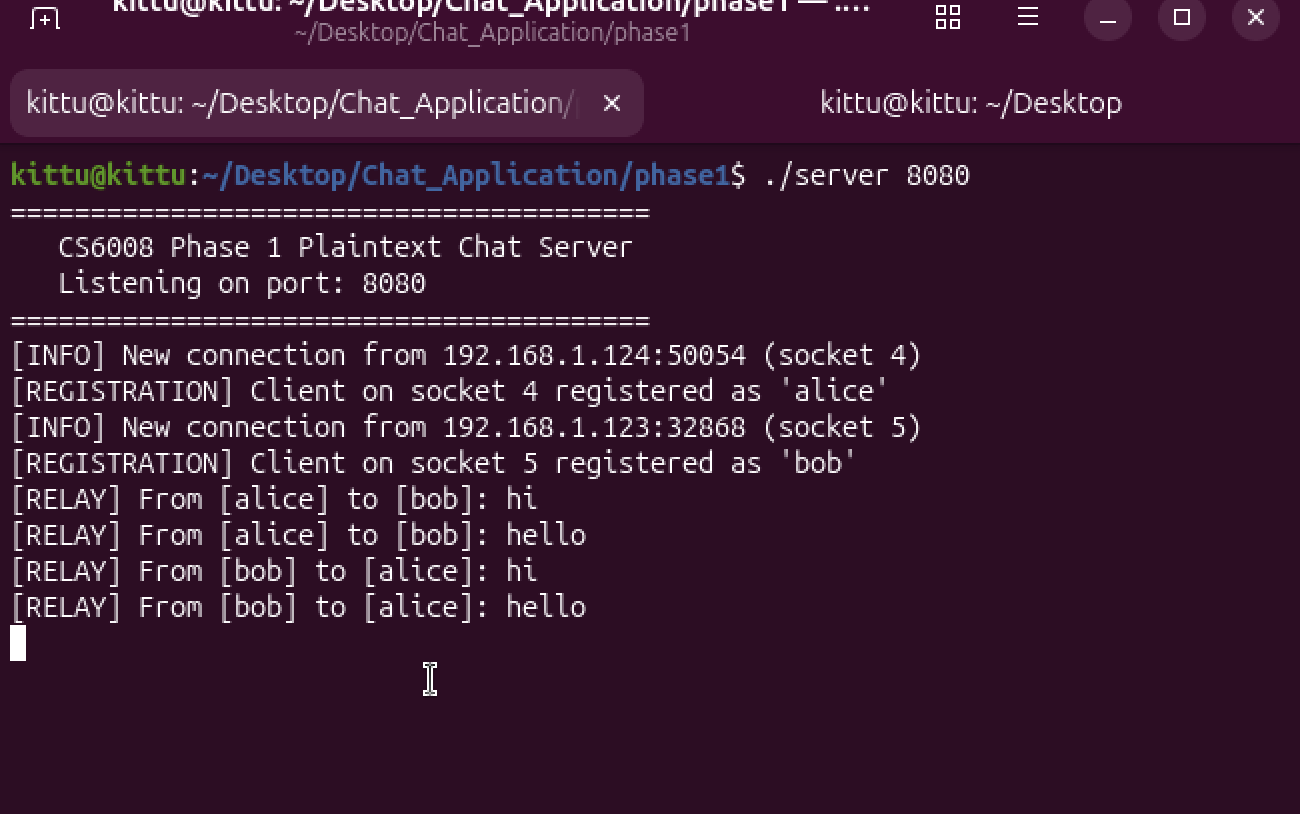
\includegraphics[width=0.72\linewidth]{phase1_server_log.png}
    \caption{Phase 1: Server terminal logging plaintext chat relays between Alice and Bob.}
    \label{fig:phase1_server}
\end{figure}

\begin{figure}[H]
    \centering
    \begin{minipage}{0.48\textwidth}
        \centering
        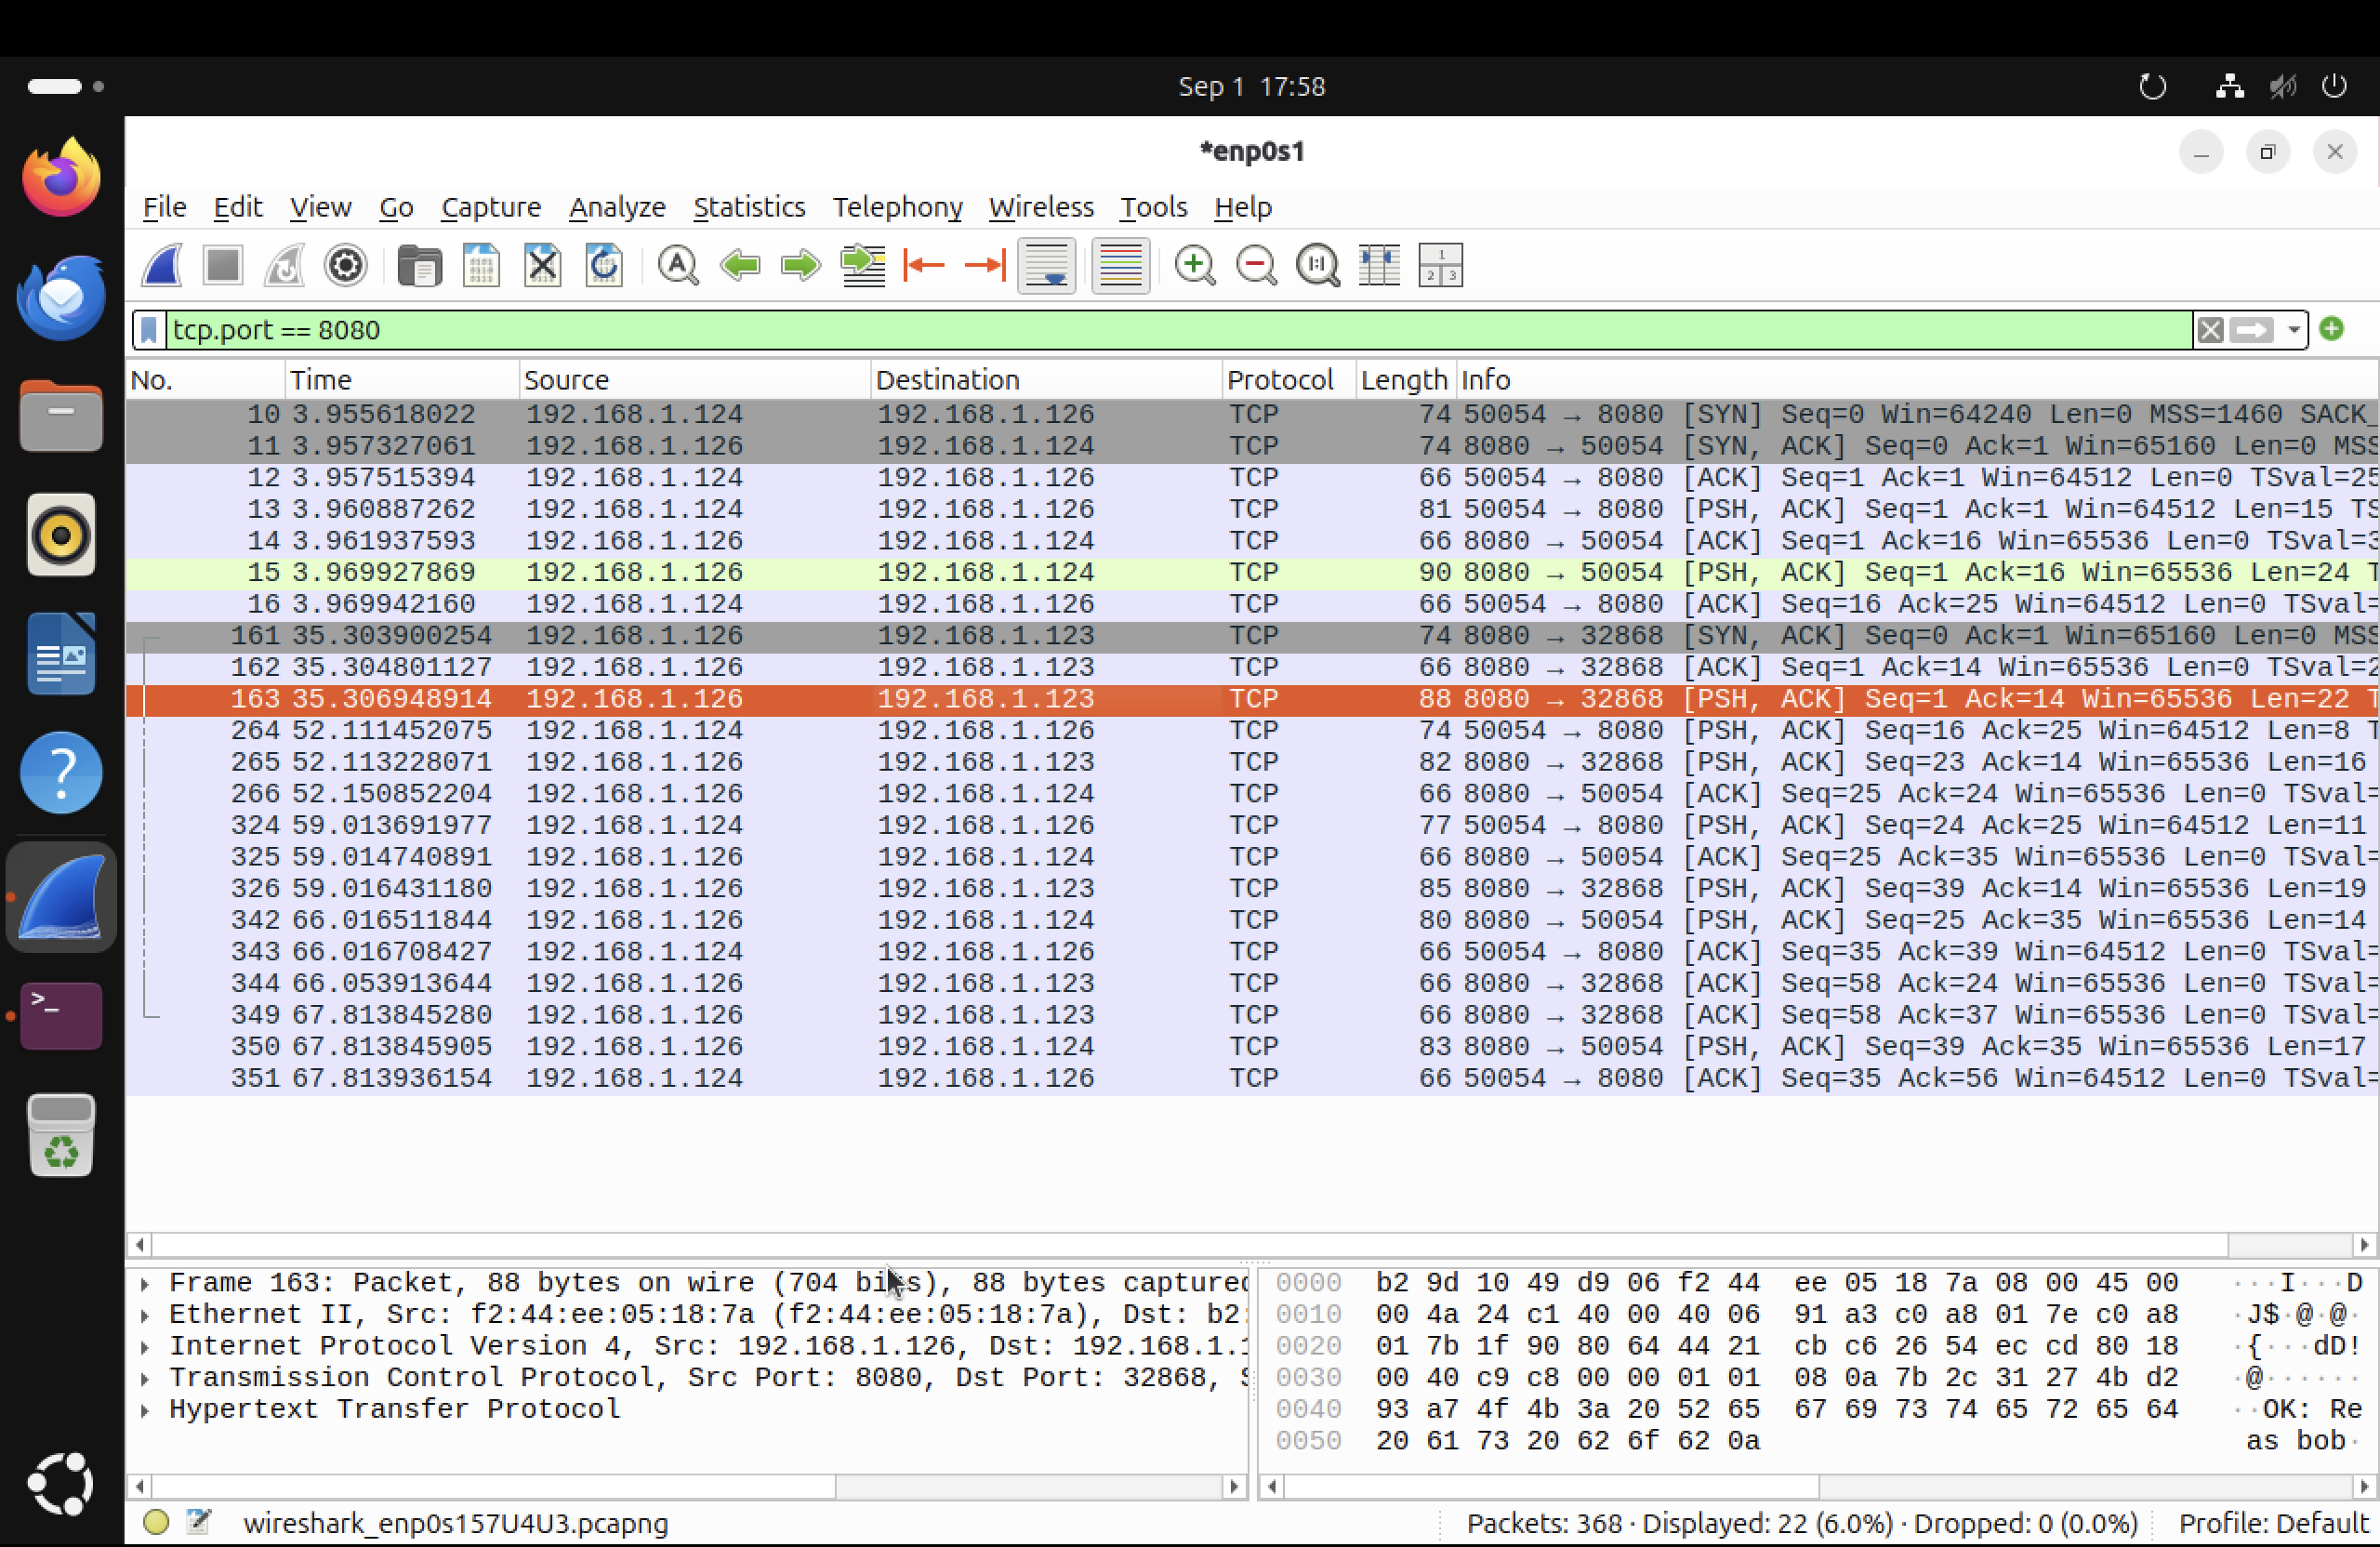
\includegraphics[width=\linewidth]{phase1_wireshark_packets.png}
        \caption{Phase 1: Wireshark capture filtered on \texttt{tcp.port == 8080}.}
        \label{fig:phase1_packets}
    \end{minipage}\hfill
    \begin{minipage}{0.48\textwidth}
        \centering
        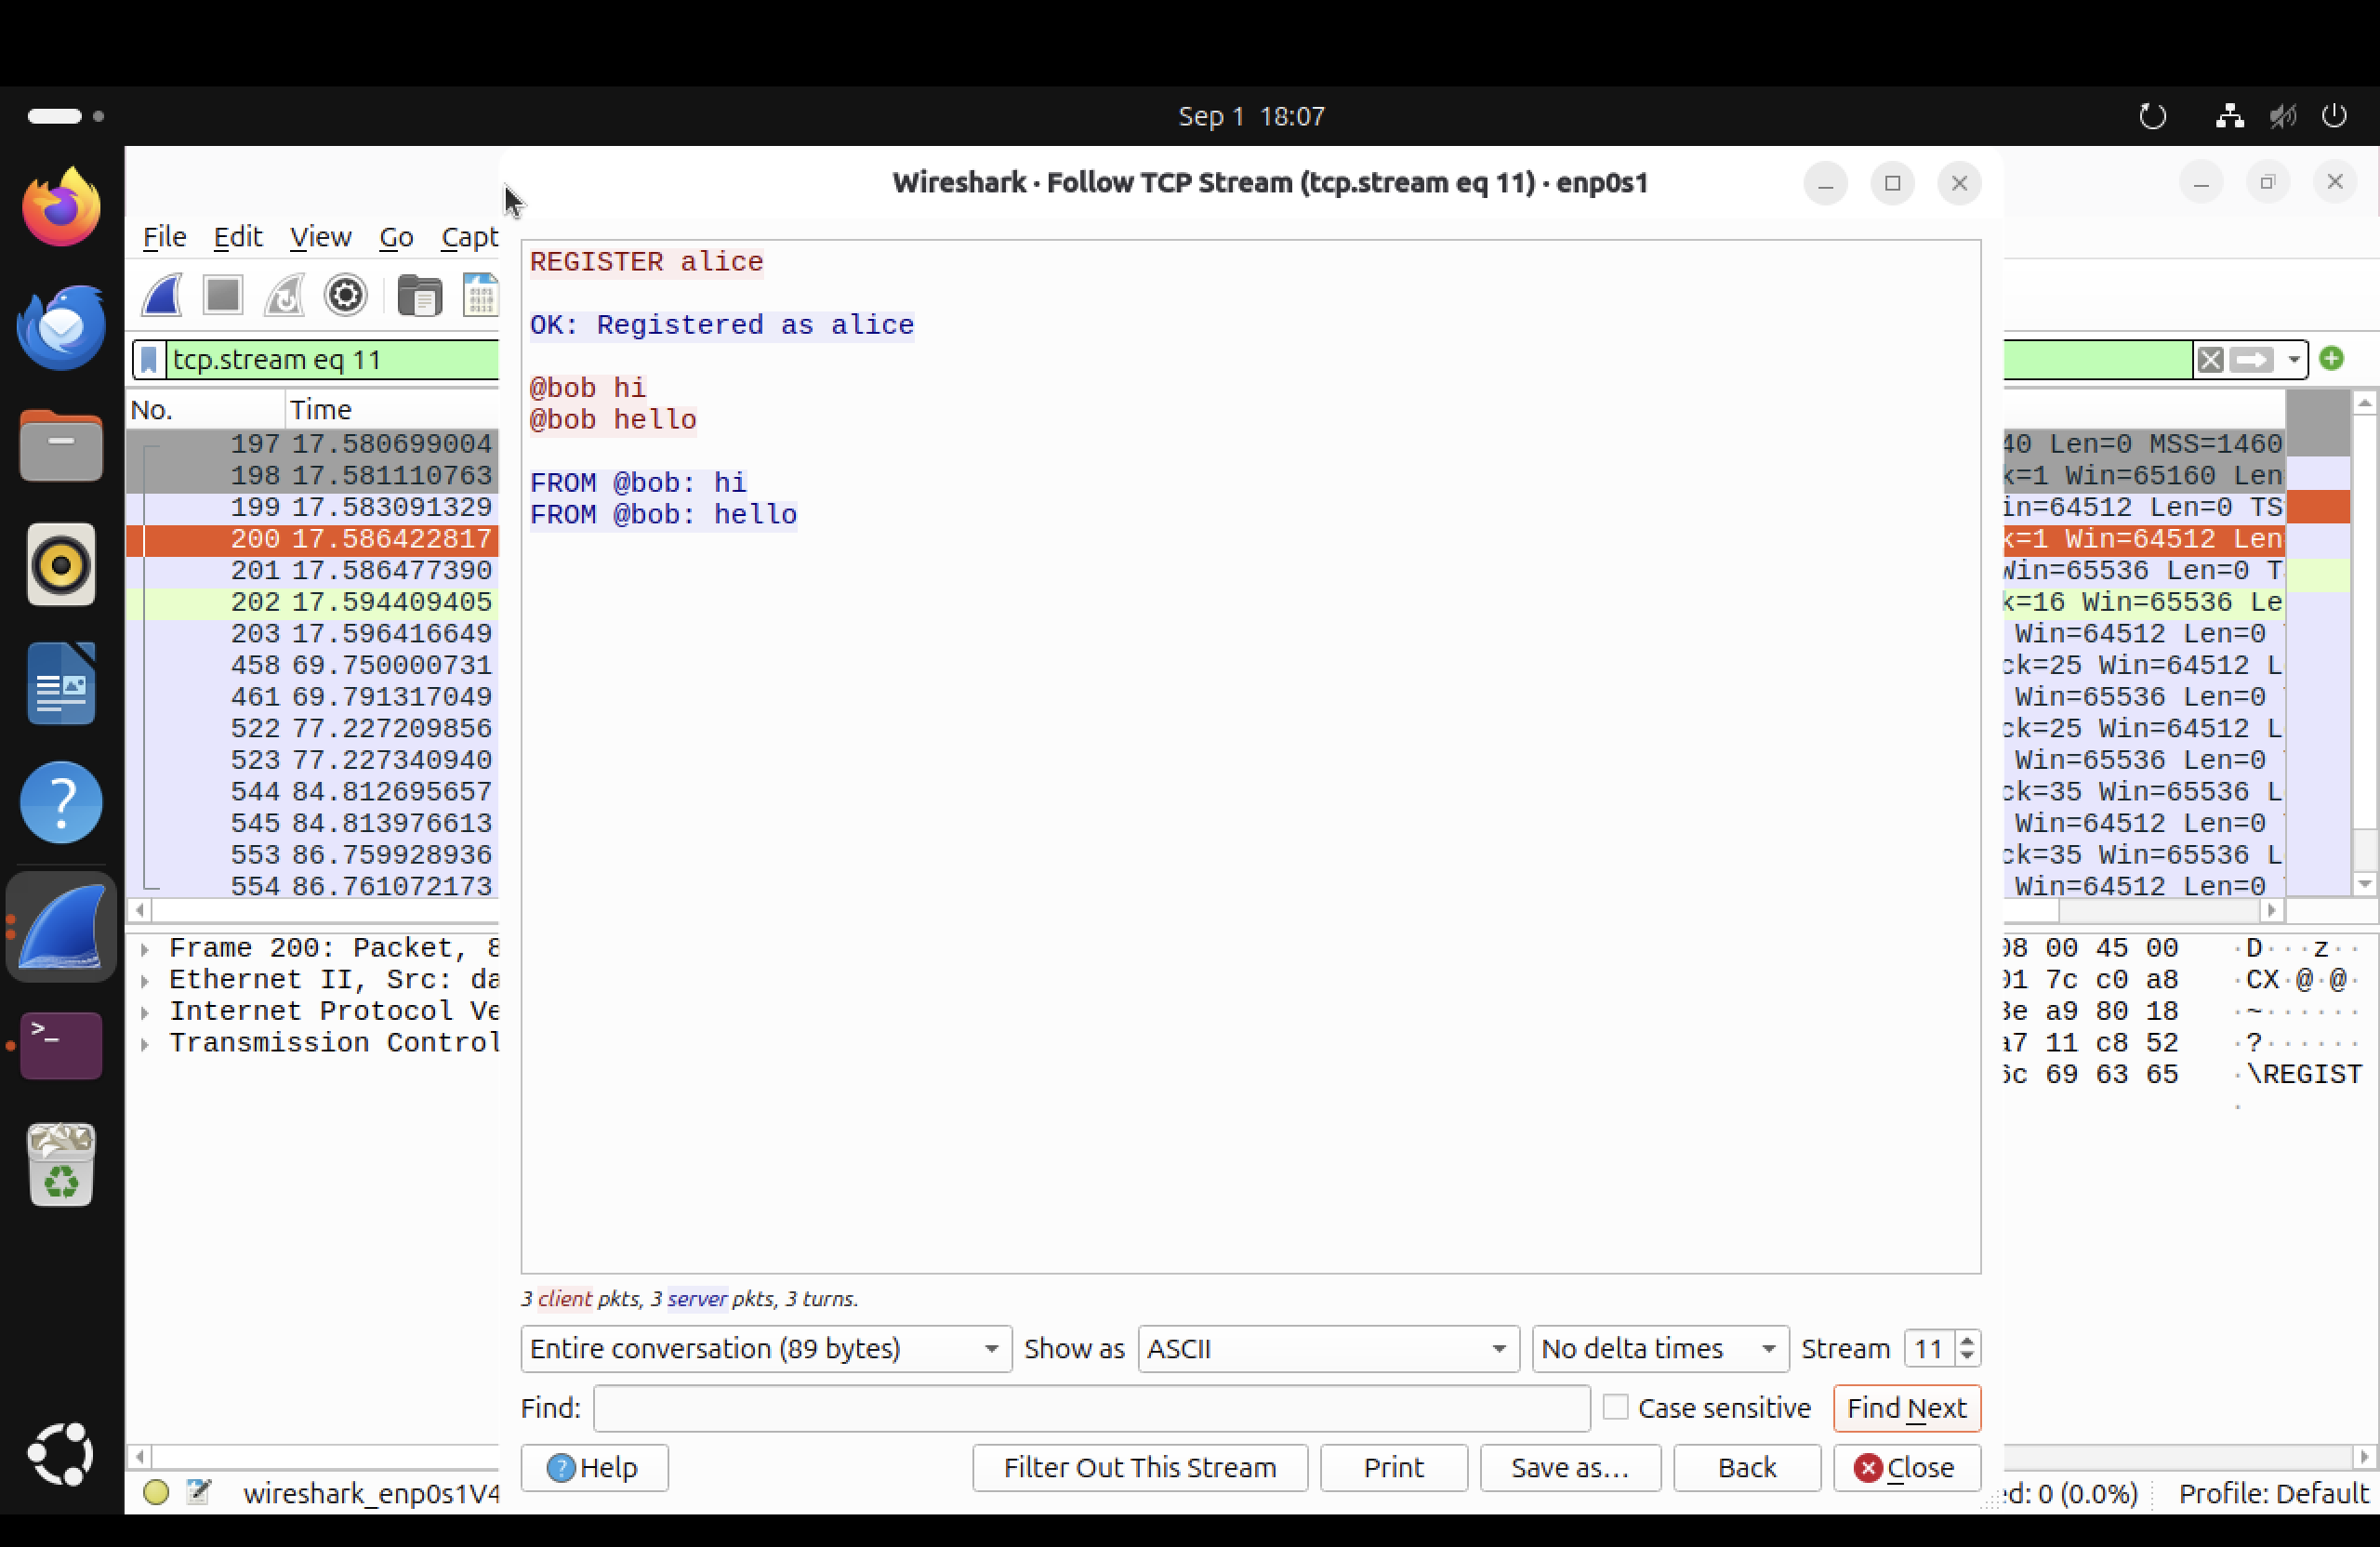
\includegraphics[width=\linewidth]{phase1_wireshark_tcp_stream.png}
        \caption{Phase 1: Wireshark Follow TCP Stream showing unencrypted text.}
        \label{fig:phase1_stream}
    \end{minipage}
\end{figure}

As shown in Figures \ref{fig:phase1_server}, \ref{fig:phase1_packets}, and \ref{fig:phase1_stream}, passive eavesdroppers and intermediate network entities have complete, uninhibited visibility into private communications and registration identifiers.

\section{Phase 2: Link Confidentiality \& MITM Attack}

\subsection{From-Scratch Diffie--Hellman Implementation}
In accordance with course rules prohibiting high-level wrapper APIs (\texttt{<openssl/ssl.h>} and \texttt{<openssl/dh.h>}), Diffie--Hellman key agreement was built from scratch using low-level BigNumber arithmetic (\texttt{<openssl/bn.h>}) on the standardized \textbf{RFC 3526 Group 14} 2048-bit MODP prime ($p$) with generator $g = 2$.

\begin{enumerate}
    \item Each party generates a cryptographically secure 2048-bit private exponent $a \in [2, p-2]$ via \texttt{BN\_rand()}.
    \item Public values $A = g^a \bmod p$ and $B = g^b \bmod p$ are computed via \texttt{BN\_mod\_exp()} and exchanged as hex strings.
    \item Both parties compute the identical raw shared secret $s = B^a \bmod p = A^b \bmod p$.
\end{enumerate}

\subsection{Cryptographic Key Derivation Function (KDF)}
\textbf{Theoretical Rationale:} The raw DH shared secret $s \in \mathbb{Z}_p^*$ cannot be used directly as an AES key. The distribution of elements produced by modular exponentiation in finite cyclic subgroups does not exhibit uniform bit entropy; certain bit positions have mathematical biases and algebraic dependencies. 

To transform the non-uniform secret into a cryptographically strong symmetric key, we apply the SHA-256 hash function as a randomness extractor:
\begin{equation}
    K_{\text{AES}} = \text{SHA-256}(s_{\text{raw}}) \in \{0,1\}^{256}
\end{equation}
The printable session key fingerprint is defined as $\text{SHA-256}(K_{\text{AES}})$.

\subsection{Authenticated Encryption: AES-256-GCM}
Unauthenticated stream or block ciphers (e.g., AES-CBC, AES-CTR) are vulnerable to bit-flipping and ciphertext tampering. We utilize AES-256 in Galois/Counter Mode (GCM) via \texttt{<openssl/evp.h>}, providing both confidentiality and data integrity. Each packet incorporates:
\begin{enumerate}
    \item A fresh 12-byte random Initialization Vector (IV) generated via \texttt{RAND\_bytes()}.
    \item Ciphertext produced via CTR mode encryption.
    \item A 16-byte Galois Message Authentication Code (GMAC) tag over $GF(2^{128})$.
\end{enumerate}

\begin{figure}[H]
    \centering
    \begin{minipage}{0.48\textwidth}
        \centering
        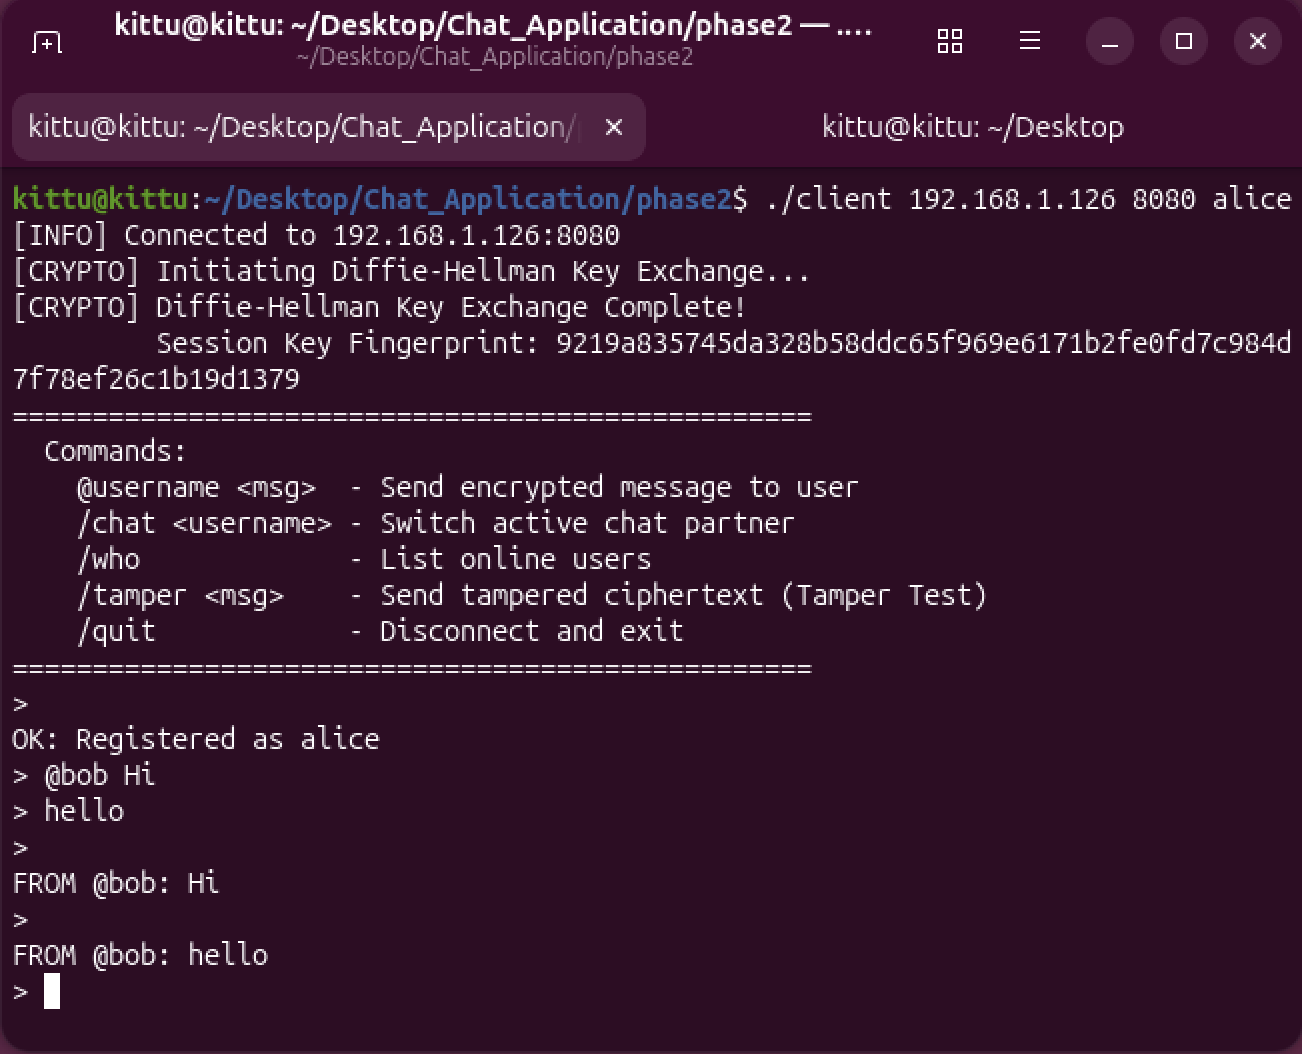
\includegraphics[width=\linewidth]{phase2_alice_normal.png}
        \caption{Phase 2: Alice client session key fingerprint.}
        \label{fig:phase2_alice}
    \end{minipage}\hfill
    \begin{minipage}{0.48\textwidth}
        \centering
        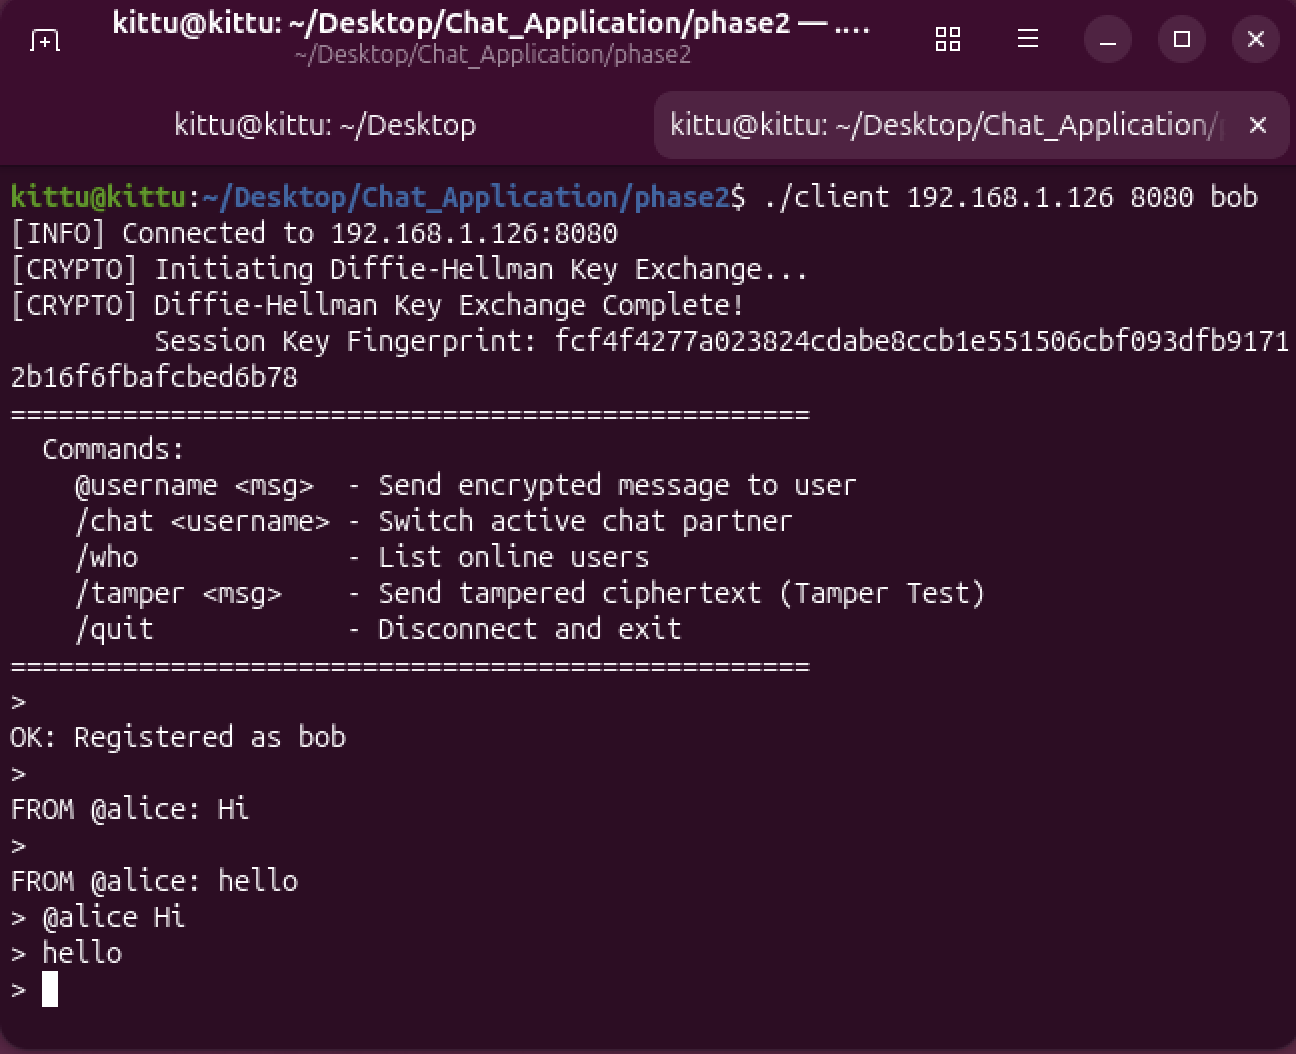
\includegraphics[width=\linewidth]{phase2_bob_normal.png}
        \caption{Phase 2: Bob client session key fingerprint.}
        \label{fig:phase2_bob}
    \end{minipage}
\end{figure}

\begin{figure}[H]
    \centering
    \begin{minipage}{0.48\textwidth}
        \centering
        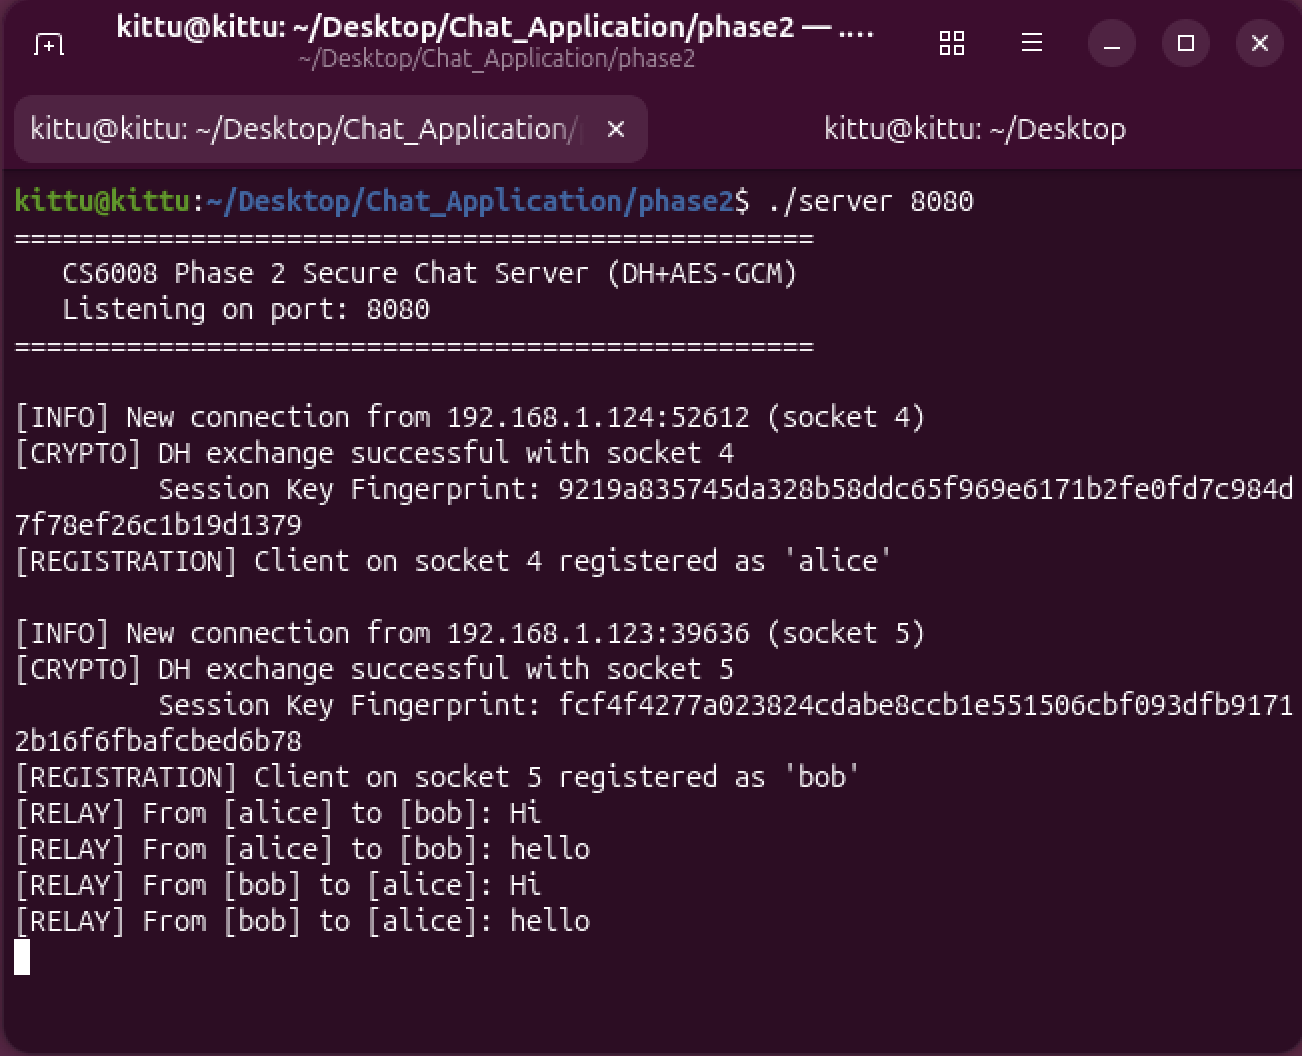
\includegraphics[width=\linewidth]{phase2_server_normal.png}
        \caption{Phase 2: Server matching session fingerprints.}
        \label{fig:phase2_server}
    \end{minipage}\hfill
    \begin{minipage}{0.48\textwidth}
        \centering
        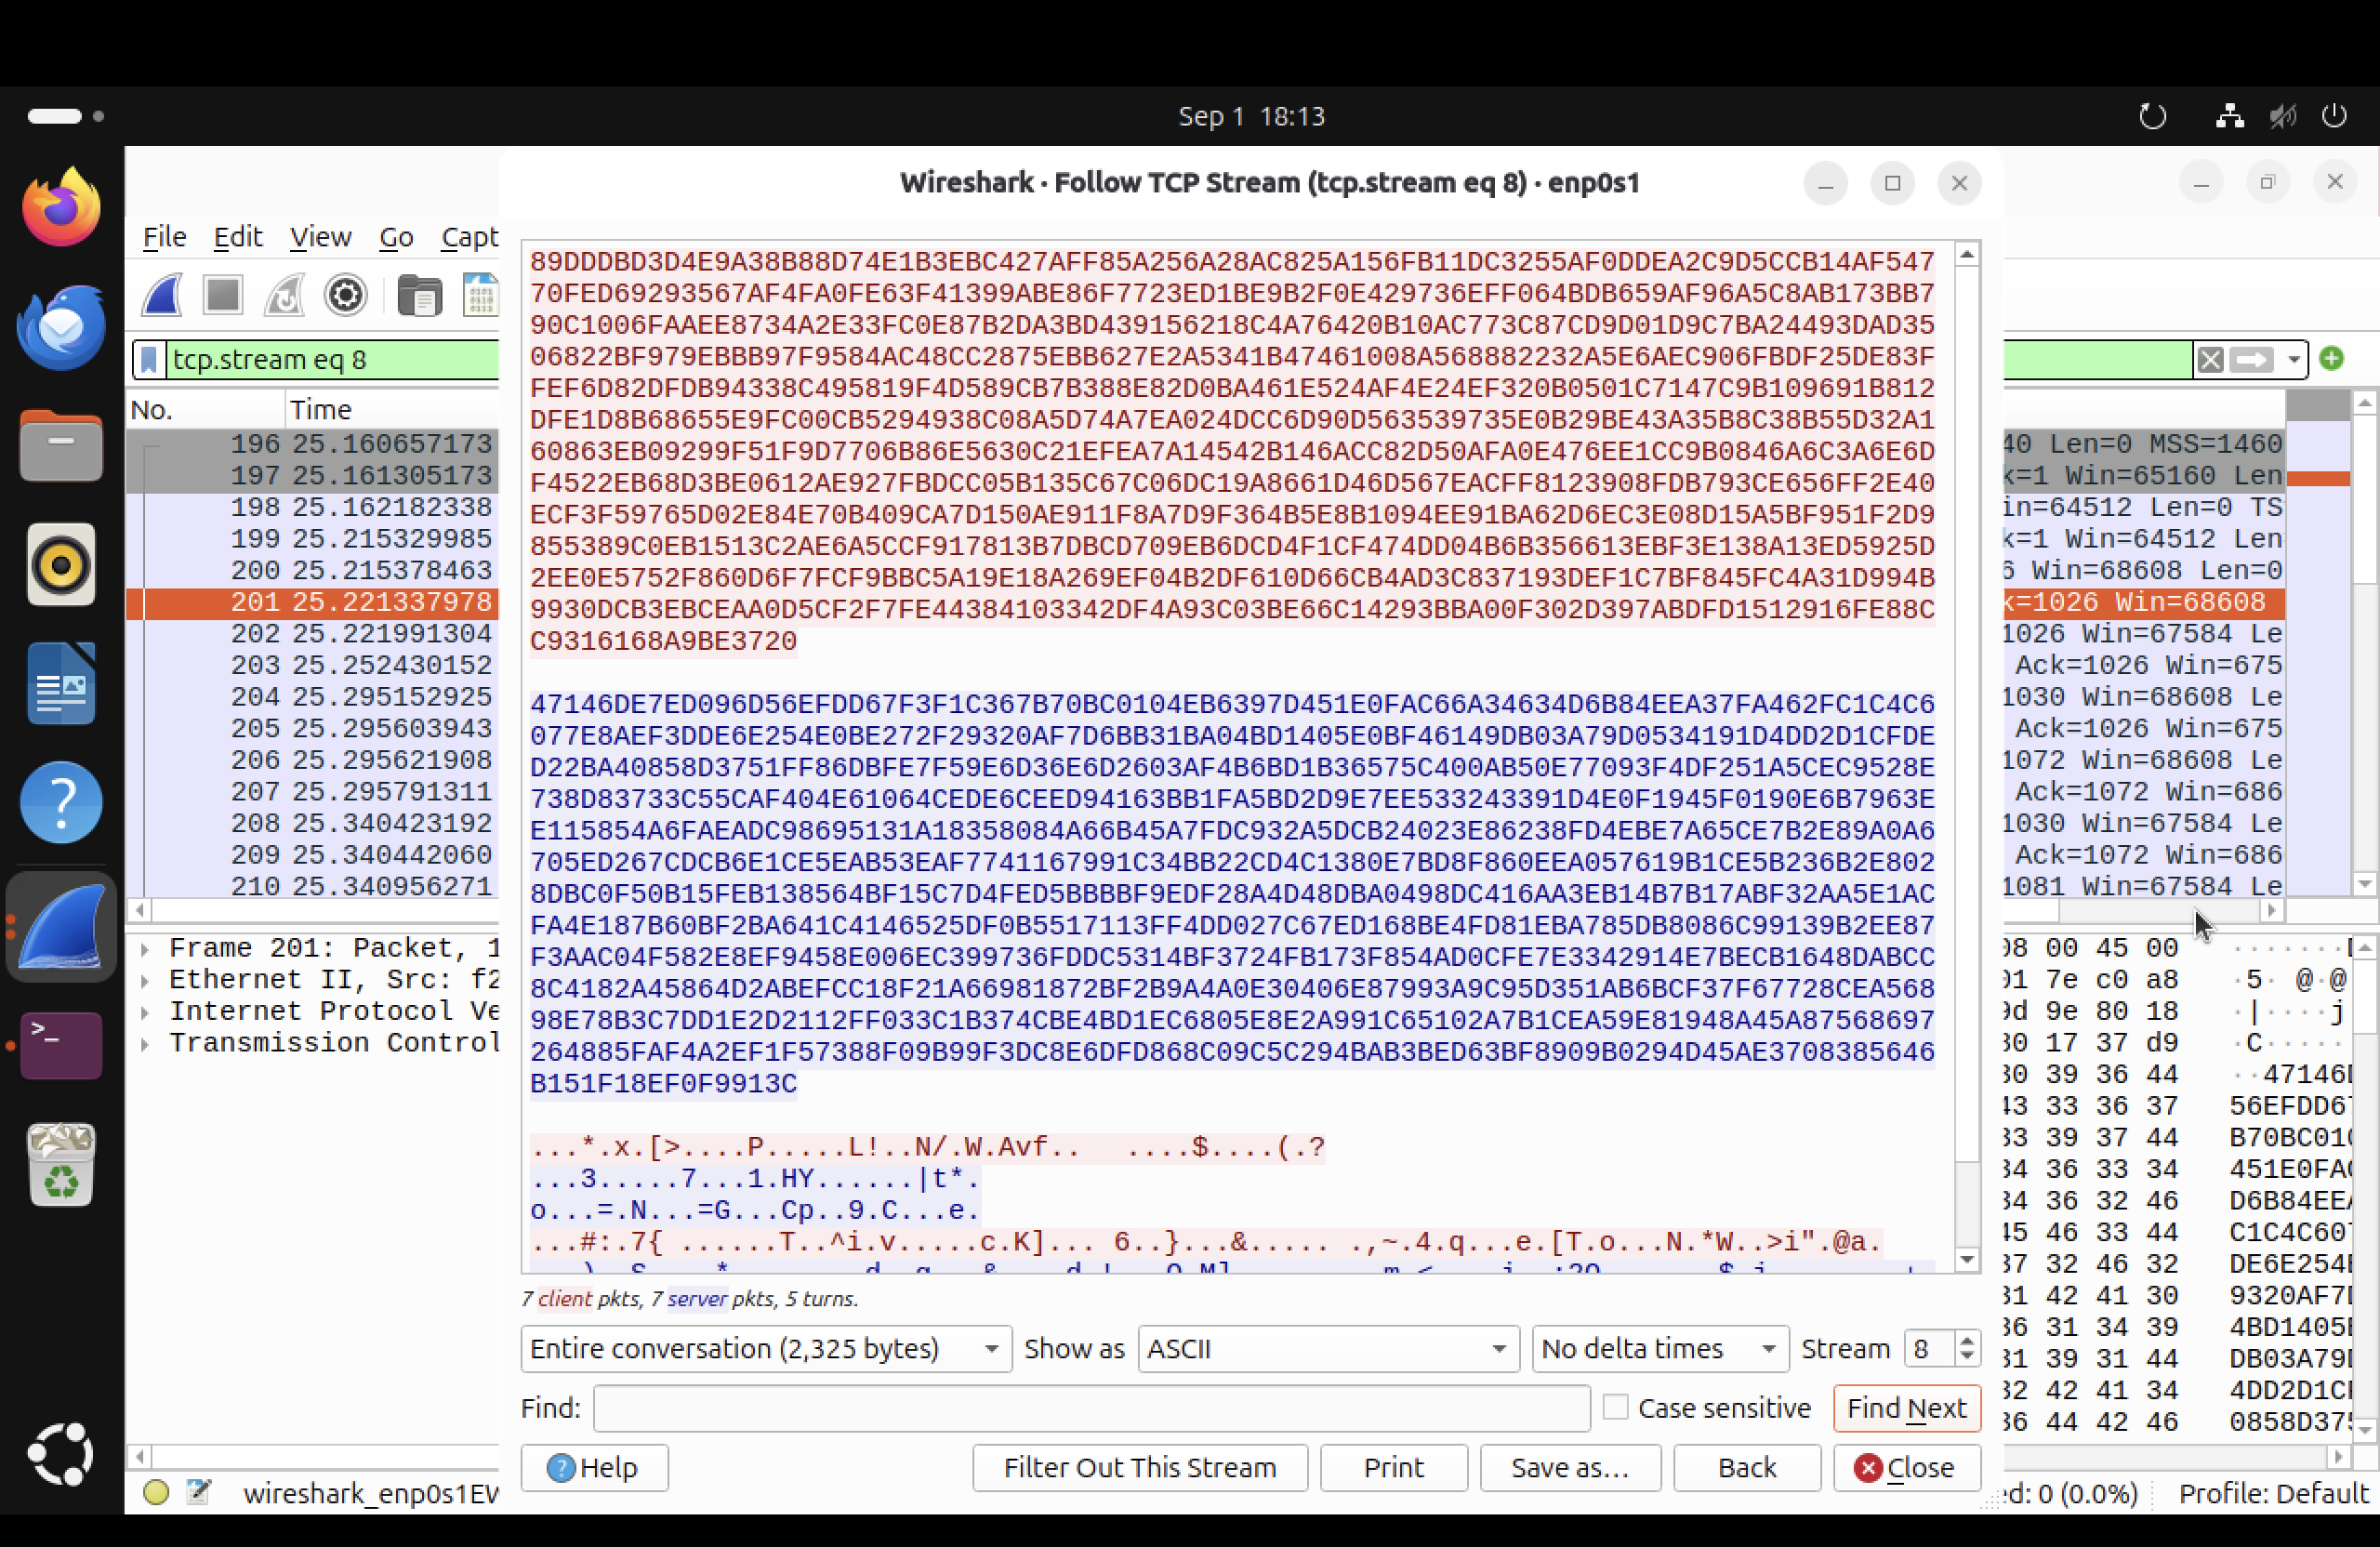
\includegraphics[width=\linewidth]{phase2_wireshark_ciphertext.png}
        \caption{Phase 2: Wireshark encrypted payload capture.}
        \label{fig:phase2_wireshark}
    \end{minipage}
\end{figure}

\subsection{Integrity Verification: Tamper Test}
A dedicated diagnostic command (\texttt{/tamper <msg>}) was implemented to flip the final byte of the ciphertext prior to wire transmission. Upon receipt, the server calls \texttt{EVP\_DecryptFinal\_ex()}, which validates the GMAC tag.

\begin{figure}[H]
    \centering
    \begin{minipage}{0.48\textwidth}
        \centering
        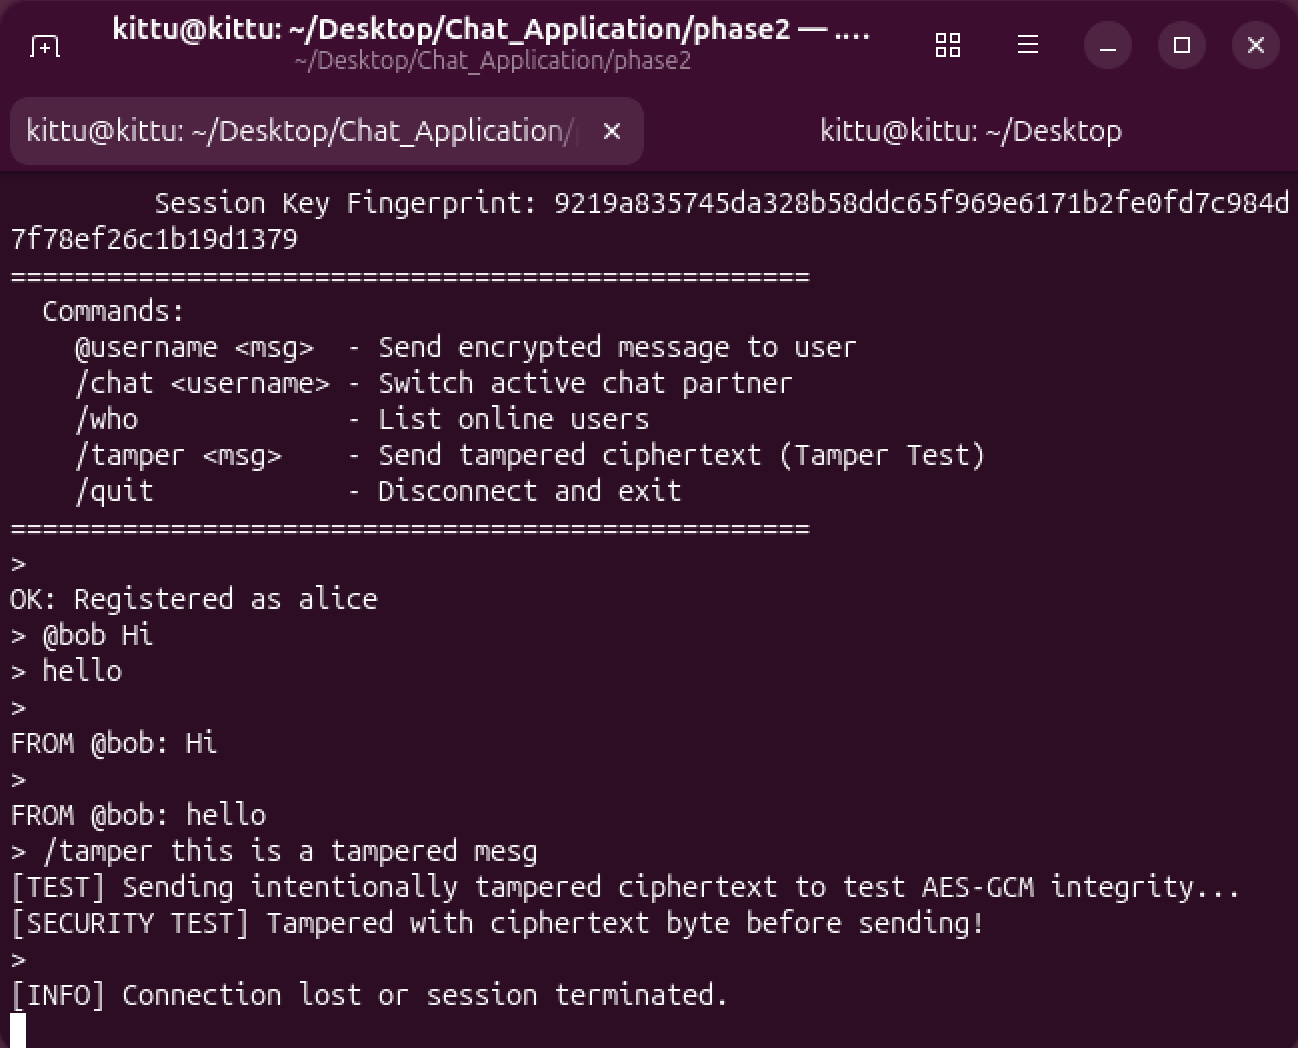
\includegraphics[width=\linewidth]{phase2_tamper_alice_client.png}
        \caption{Phase 2: Alice executing \texttt{/tamper} command.}
        \label{fig:phase2_tamper_alice}
    \end{minipage}\hfill
    \begin{minipage}{0.48\textwidth}
        \centering
        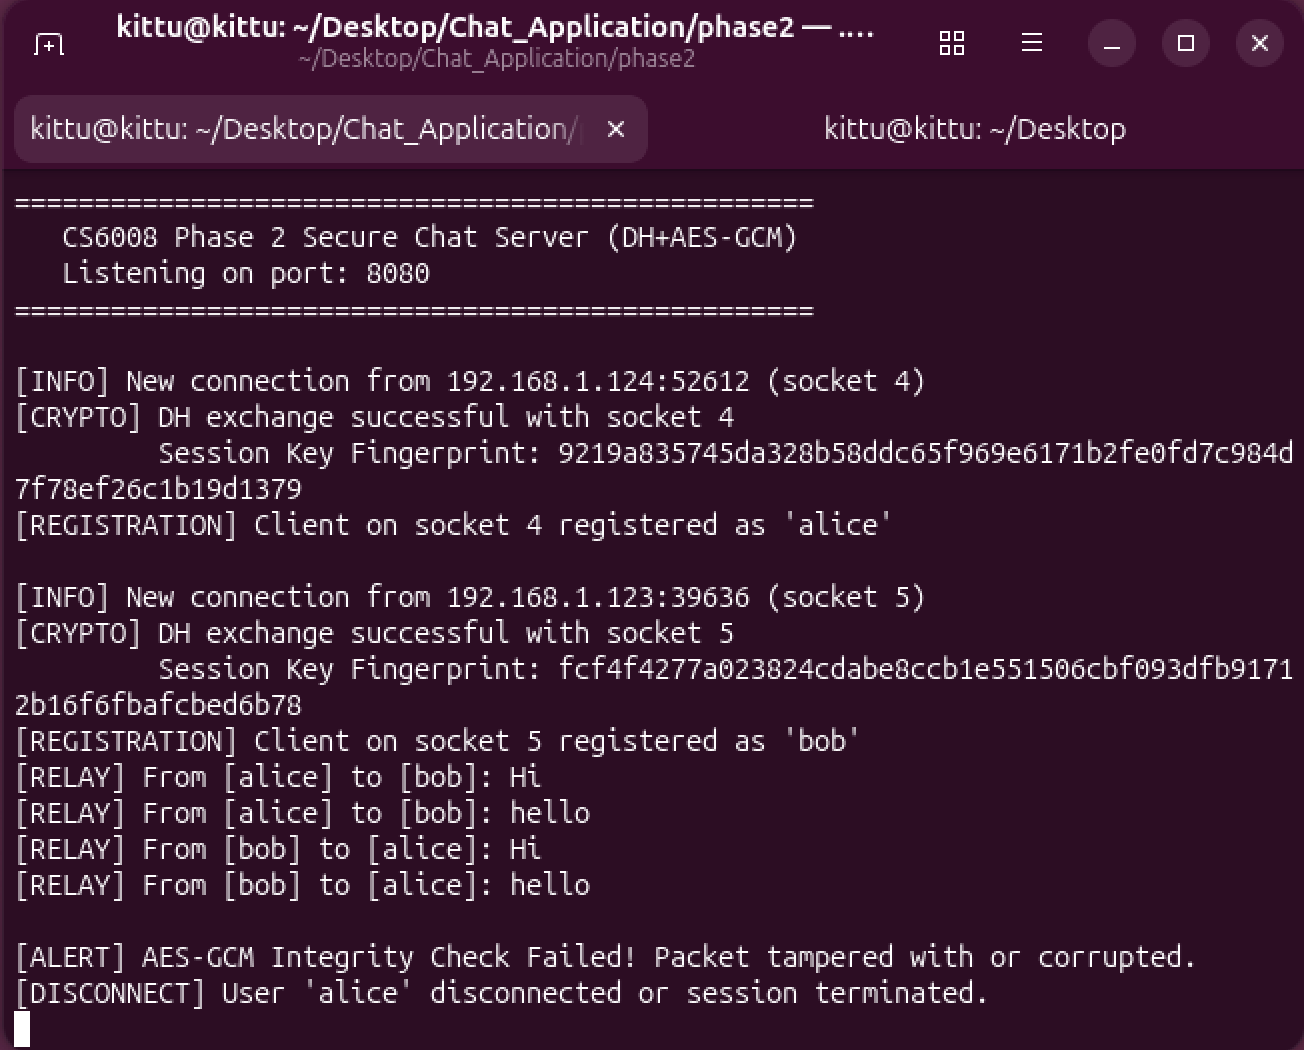
\includegraphics[width=\linewidth]{phase2_tamper_server_alert.png}
        \caption{Phase 2: Server rejecting tampered ciphertext.}
        \label{fig:phase2_tamper_server}
    \end{minipage}
\end{figure}

As shown in Figure \ref{fig:phase2_tamper_server}, the server immediately flags \texttt{[ALERT] AES-GCM Integrity Check Failed!} and terminates the compromised socket, preventing forged or manipulated payloads.

\subsection{The Man-in-the-Middle (MITM) Attack}
Because unauthenticated Diffie--Hellman exchanges public keys in the clear without cryptographic binding to node identities, an active attacker positioned on the network path can intercept and split the key exchange.

We implemented an active MITM proxy tool (\texttt{mallory\_proxy}). When Alice connects to Mallory (believing Mallory is the server), Mallory establishes two distinct, independent DH handshakes:
\begin{enumerate}
    \item Handshake 1 ($C1 \leftrightarrow M$): Negotiates Key $K_1$.
    \item Handshake 2 ($M \leftrightarrow S$): Negotiates Key $K_2$.
\end{enumerate}
When Alice sends a message encrypted under $K_1$, Mallory decrypts it to plaintext, logs it, re-encrypts under $K_2$, and forwards it to the Server.

\begin{figure}[H]
    \centering
    \begin{minipage}{0.48\textwidth}
        \centering
        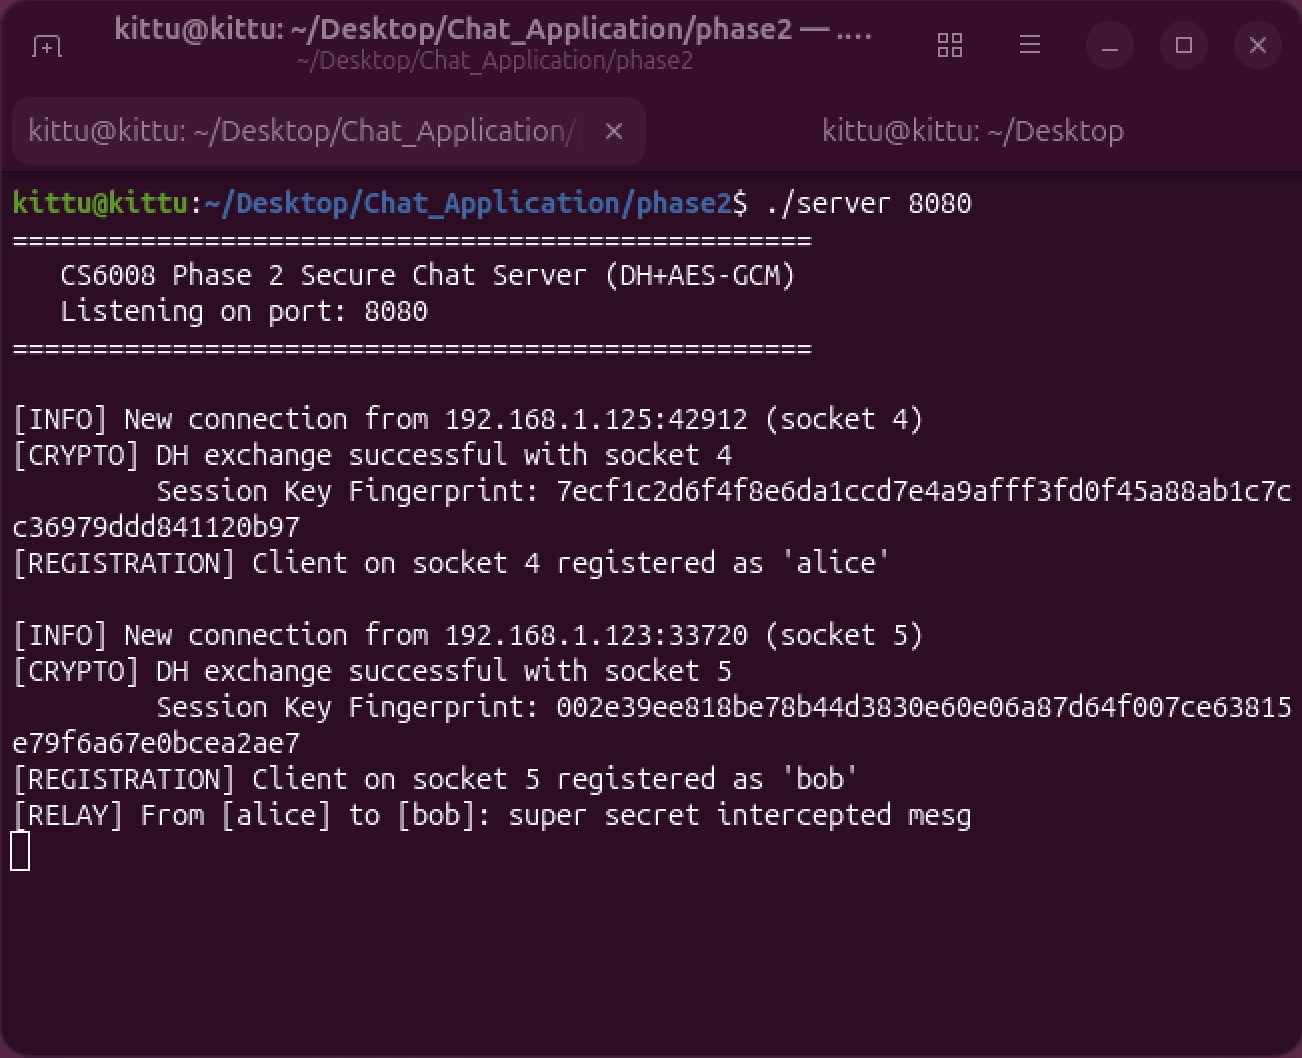
\includegraphics[width=\linewidth]{phase2_mitm_alice_client.png}
        \caption{Phase 2: Server communicating with Mallory.}
        \label{fig:phase2_mitm_alice}
    \end{minipage}\hfill
    \begin{minipage}{0.48\textwidth}
        \centering
        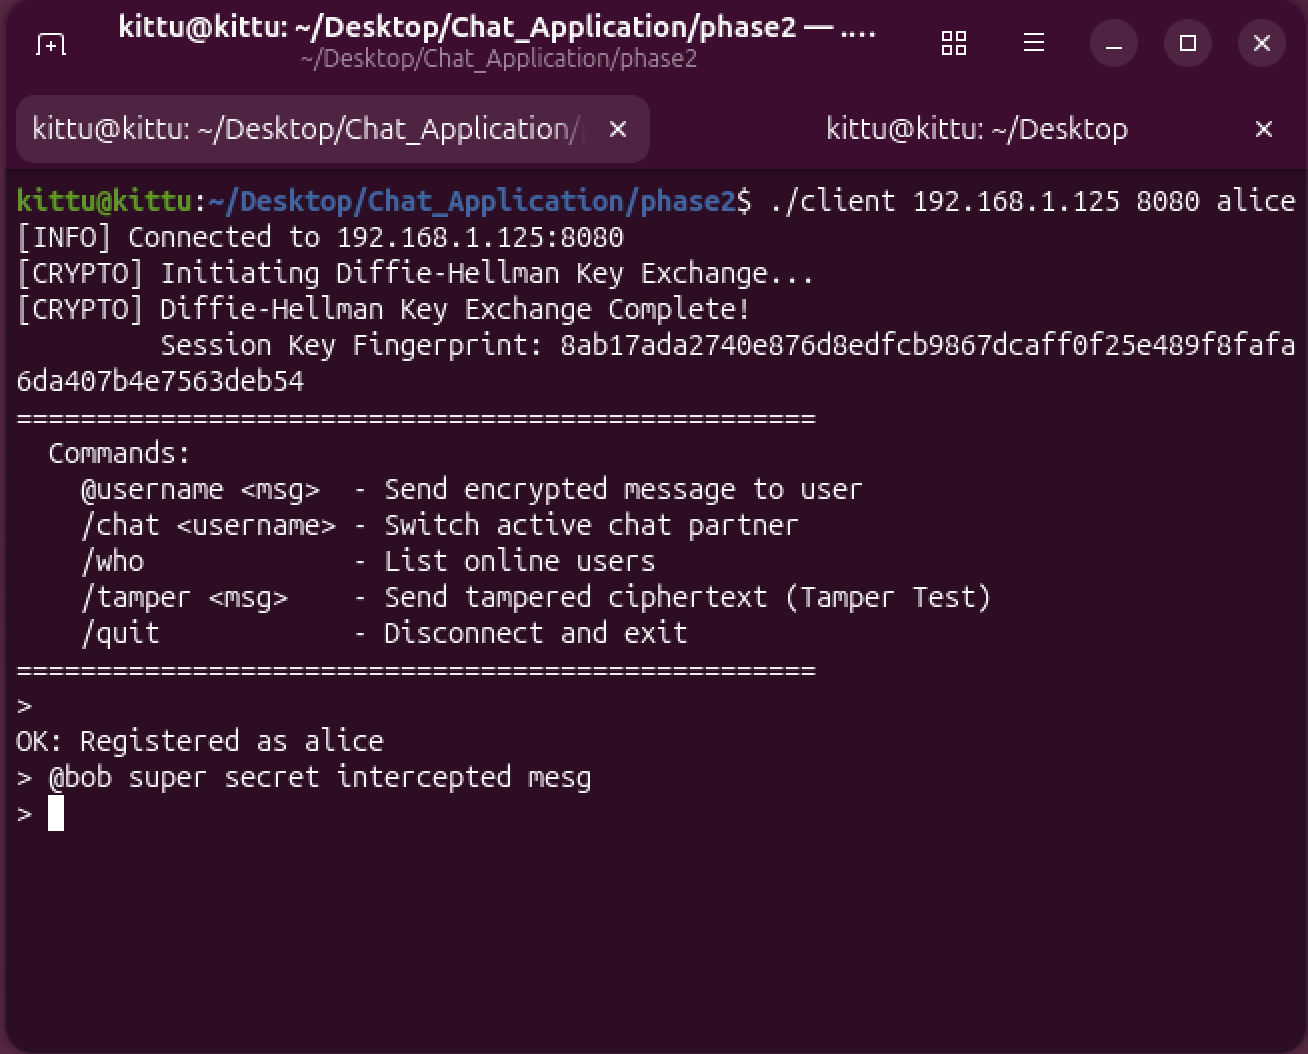
\includegraphics[width=\linewidth]{phase2_mitm_bob_client.png}
        \caption{Phase 2: Alice connected through Mallory proxy.}
        \label{fig:phase2_mitm_bob}
    \end{minipage}
\end{figure}

\begin{figure}[H]
    \centering
    \begin{minipage}{0.48\textwidth}
        \centering
        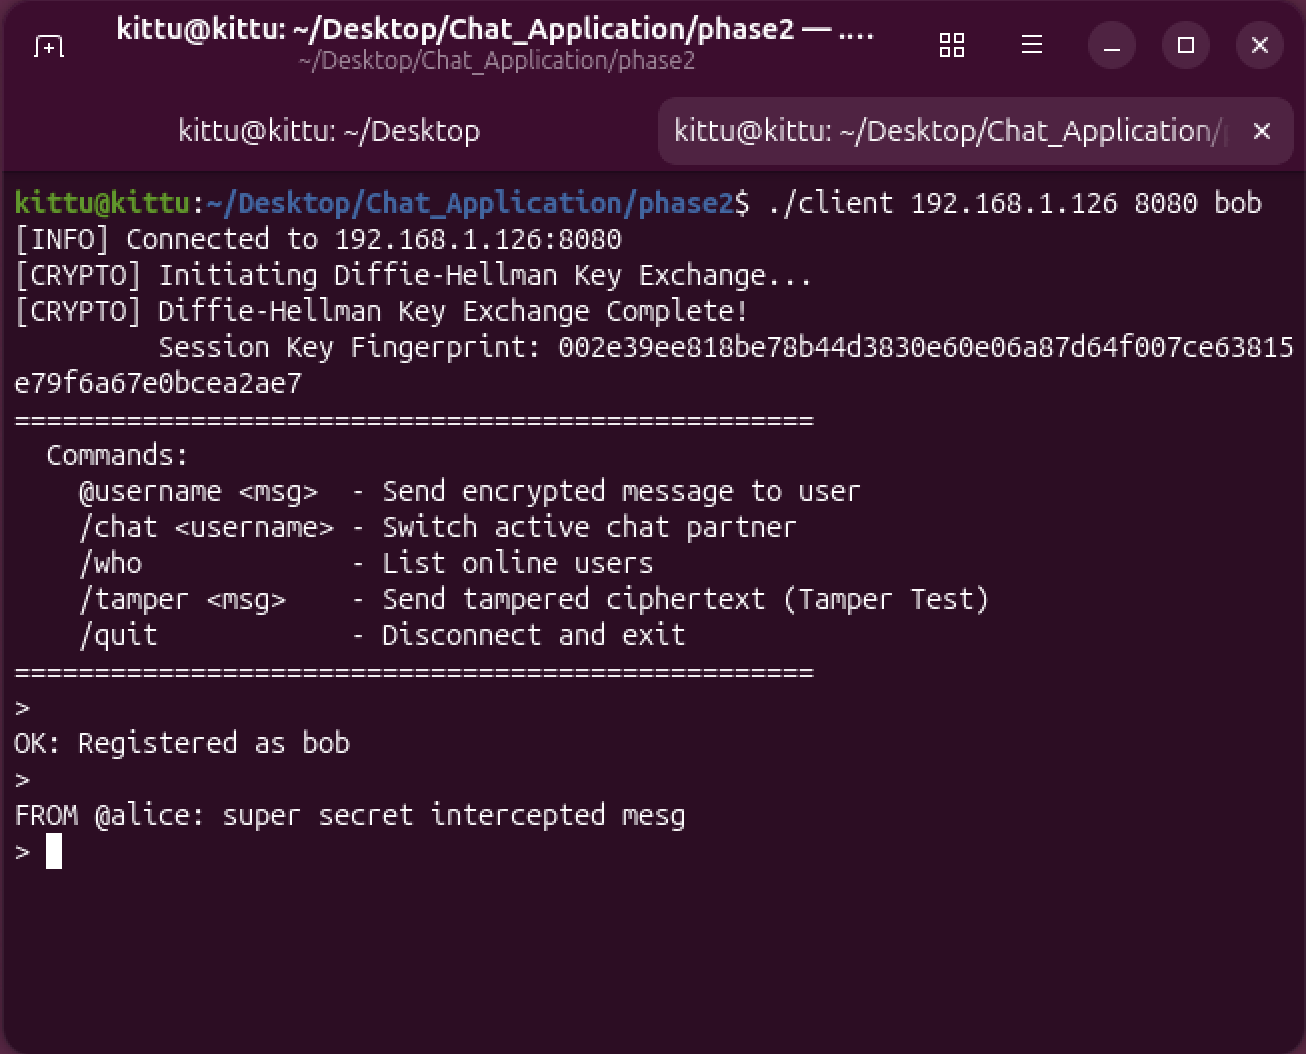
\includegraphics[width=\linewidth]{phase2_mitm_server.png}
        \caption{Phase 2: Bob connected to Server.}
        \label{fig:phase2_mitm_server}
    \end{minipage}\hfill
    \begin{minipage}{0.48\textwidth}
        \centering
        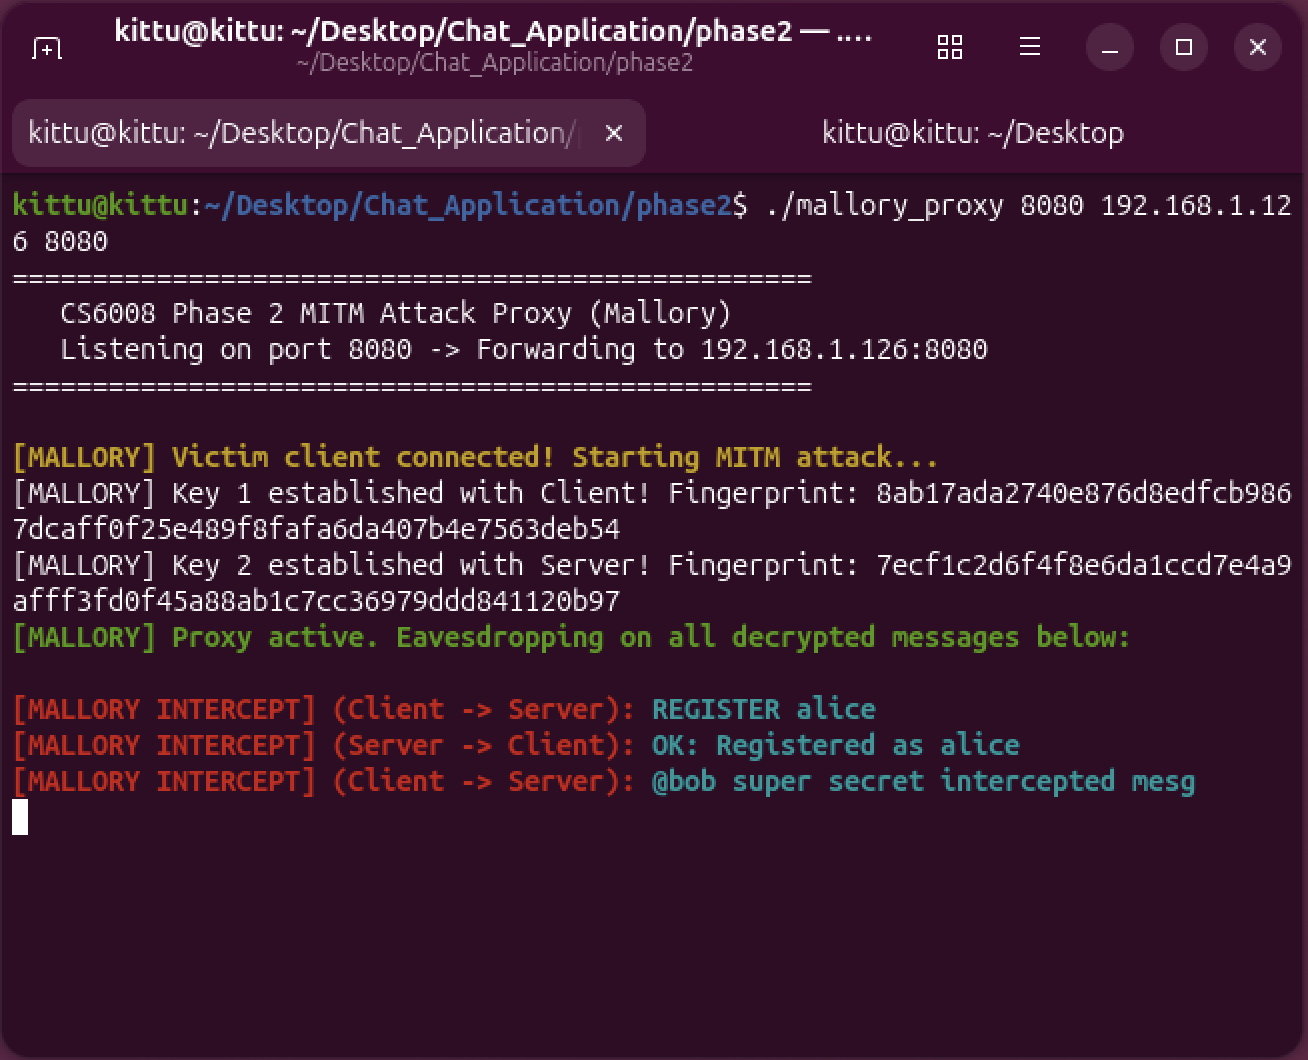
\includegraphics[width=\linewidth]{phase2_mitm_mallory_intercept.png}
        \caption{Phase 2: Mallory intercepting cleartext chat.}
        \label{fig:phase2_mitm_mallory}
    \end{minipage}
\end{figure}

\noindent\textbf{Observable Evidence of Compromise:} An ordinary user typing chat messages has no visual cue of the attack since messages are delivered seamlessly. However, the attack is detectable by comparing session key fingerprints:
\begin{itemize}
    \item Alice Key Fingerprint: \texttt{8ab17ada2740...} (matches Mallory $K_1$).
    \item Server Key Fingerprint: \texttt{7ecf1c2d6f4f...} (matches Mallory $K_2$).
\end{itemize}
The disparity between Alice's fingerprint and the Server's fingerprint is definitive mathematical proof of an active MITM interception.

\section{Phase 3: PKI Authentication \& Proof-of-Possession}

\subsection{Public Key Infrastructure (PKI) Setup}
To defeat the MITM vulnerability exposed in Phase 2, we established a Public Key Infrastructure using OpenSSL:
\begin{enumerate}
    \item \textbf{Root CA:} A self-signed Root Certificate Authority (\texttt{ca.crt}) with 4096-bit RSA key (\texttt{ca.key}) was generated.
    \item \textbf{Server Certificate:} The chat server generated a 2048-bit RSA private key (\texttt{server.key}) and a Certificate Signing Request (CSR) with Common Name $\text{CN} = \texttt{chat.server.local}$. The CSR was signed by the Root CA to produce \texttt{server.crt}.
\end{enumerate}

\begin{figure}[H]
    \centering
    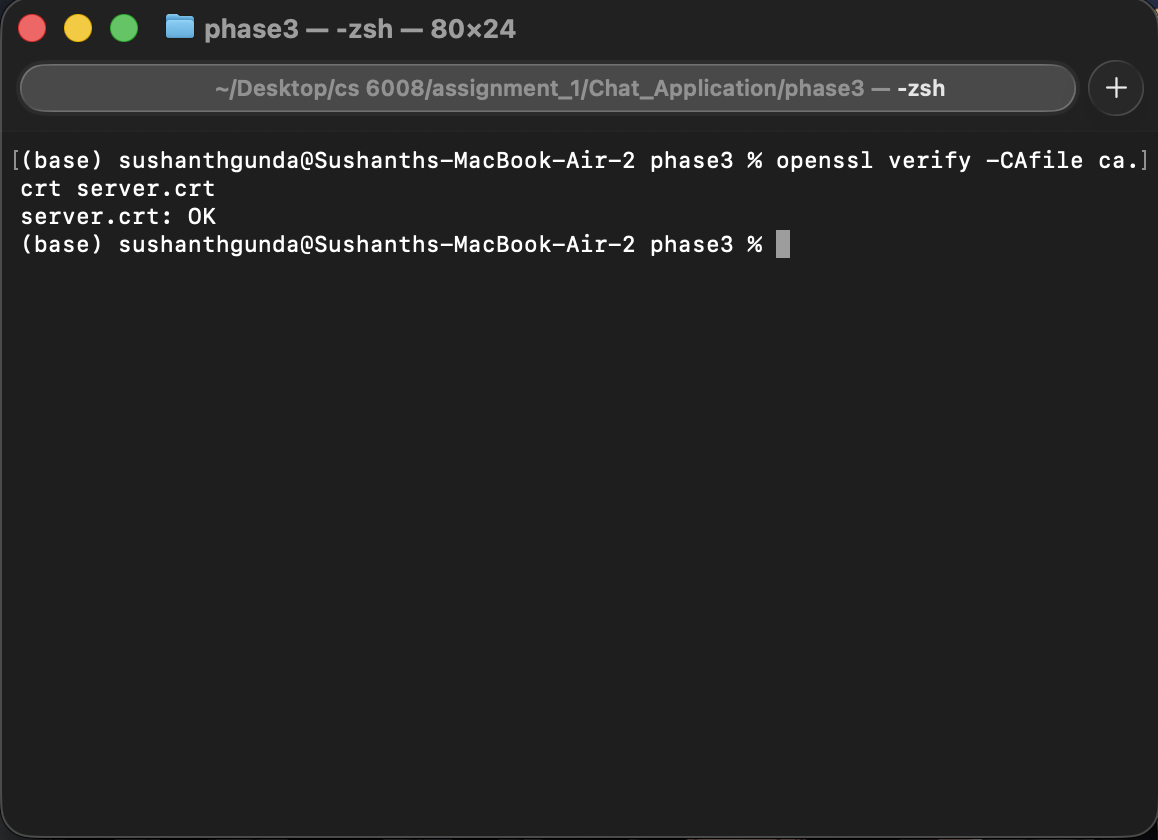
\includegraphics[width=0.6\linewidth]{phase3_openssl_verify_cli.png}
    \caption{Phase 3: OpenSSL CLI validation of Server certificate against Root CA.}
    \label{fig:phase3_cli}
\end{figure}

\subsection{Client Certificate Validation Chain}
During connection initiation, the server sends its PEM-encoded \texttt{server.crt}. The client verifies the certificate using \texttt{<openssl/x509.h>} by checking:
\begin{enumerate}
    \item \textbf{Signature Validity:} Verified against the trusted local \texttt{ca.crt} via \texttt{X509\_verify\_cert()}.
    \item \textbf{Temporal Validity:} Checks \texttt{notBefore} and \texttt{notAfter}.
    \item \textbf{Identity Binding:} Confirms $\text{Subject CN} == \texttt{chat.server.local}$.
\end{enumerate}

\subsection{Vouched Identity vs. Proof-of-Possession (PoP)}
\textbf{Theoretical Rationale:} Certificate validation alone only proves that \texttt{server.crt} is a valid document issued by the trusted CA. Because public certificates are openly distributable, an attacker could steal \texttt{server.crt} and replay it to clients. 

To prove that the remote party actually owns the matching private key, we implement a dynamic Proof-of-Possession challenge-response handshake:
\begin{enumerate}
    \item Client generates a cryptographically random 32-byte nonce $N_{\text{client}}$ and sends it to the server.
    \item Server signs the concatenated challenge $(N_{\text{client}} \mathbin{\Vert} \text{DH\_Pub}_{\text{Server}})$ using its RSA private key via \texttt{EVP\_DigestSign} (RSA-SHA256).
    \item Client extracts the public key from \texttt{server.crt} and verifies the signature using \texttt{EVP\_DigestVerify}.
\end{enumerate}
Signing the server's ephemeral DH public key inside the challenge firmly binds the key exchange to the authenticated server identity.

\begin{figure}[H]
    \centering
    \begin{minipage}{0.48\textwidth}
        \centering
        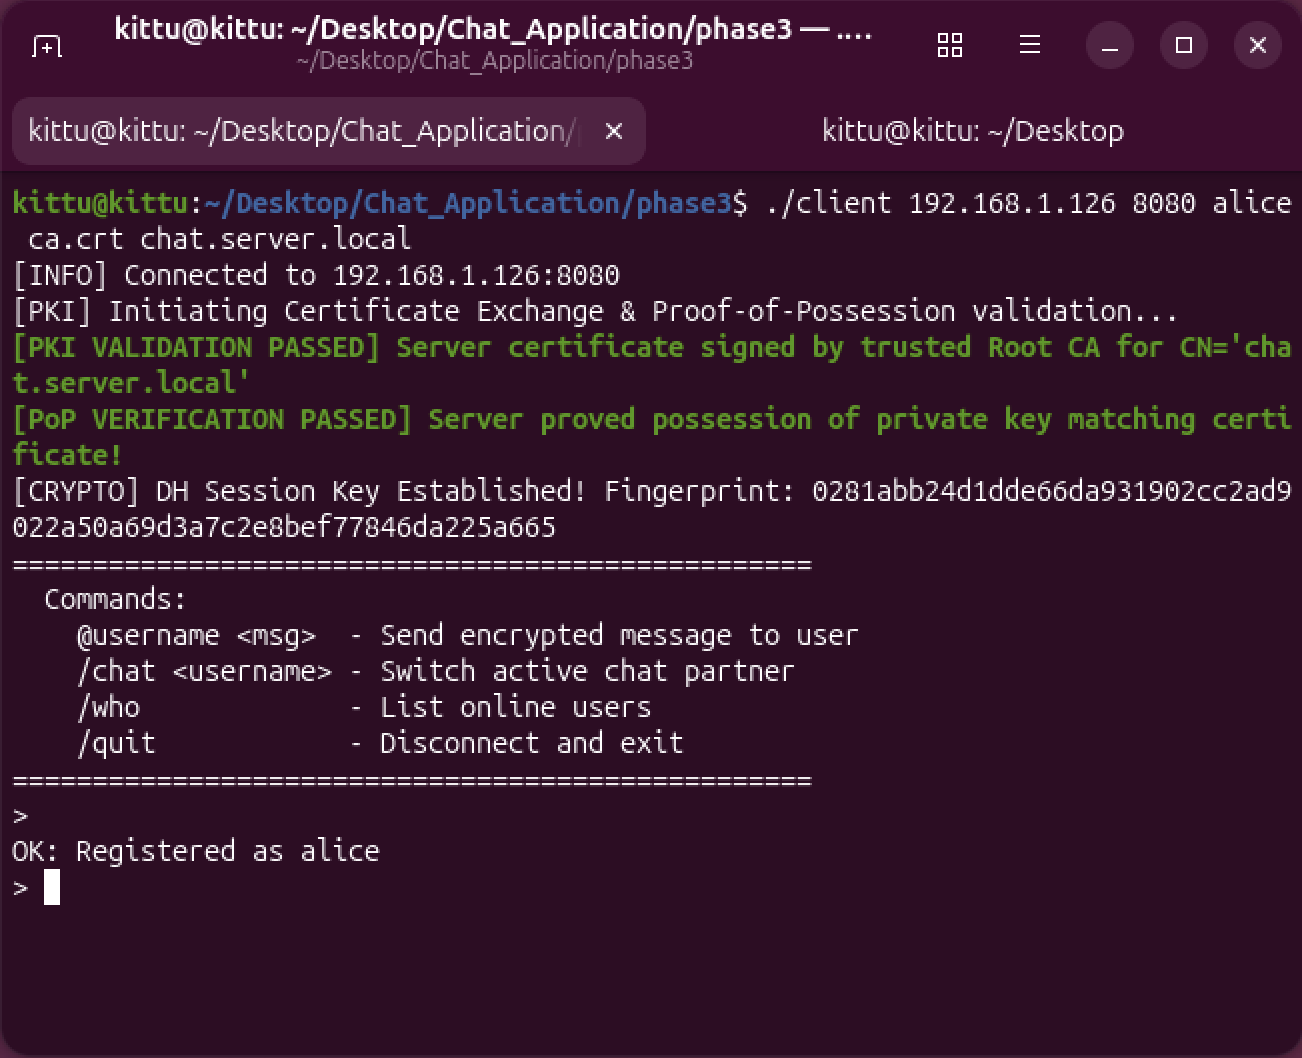
\includegraphics[width=\linewidth]{phase3_legitimate_client.png}
        \caption{Phase 3: Client validating PKI \& PoP.}
        \label{fig:phase3_legit_client}
    \end{minipage}\hfill
    \begin{minipage}{0.48\textwidth}
        \centering
        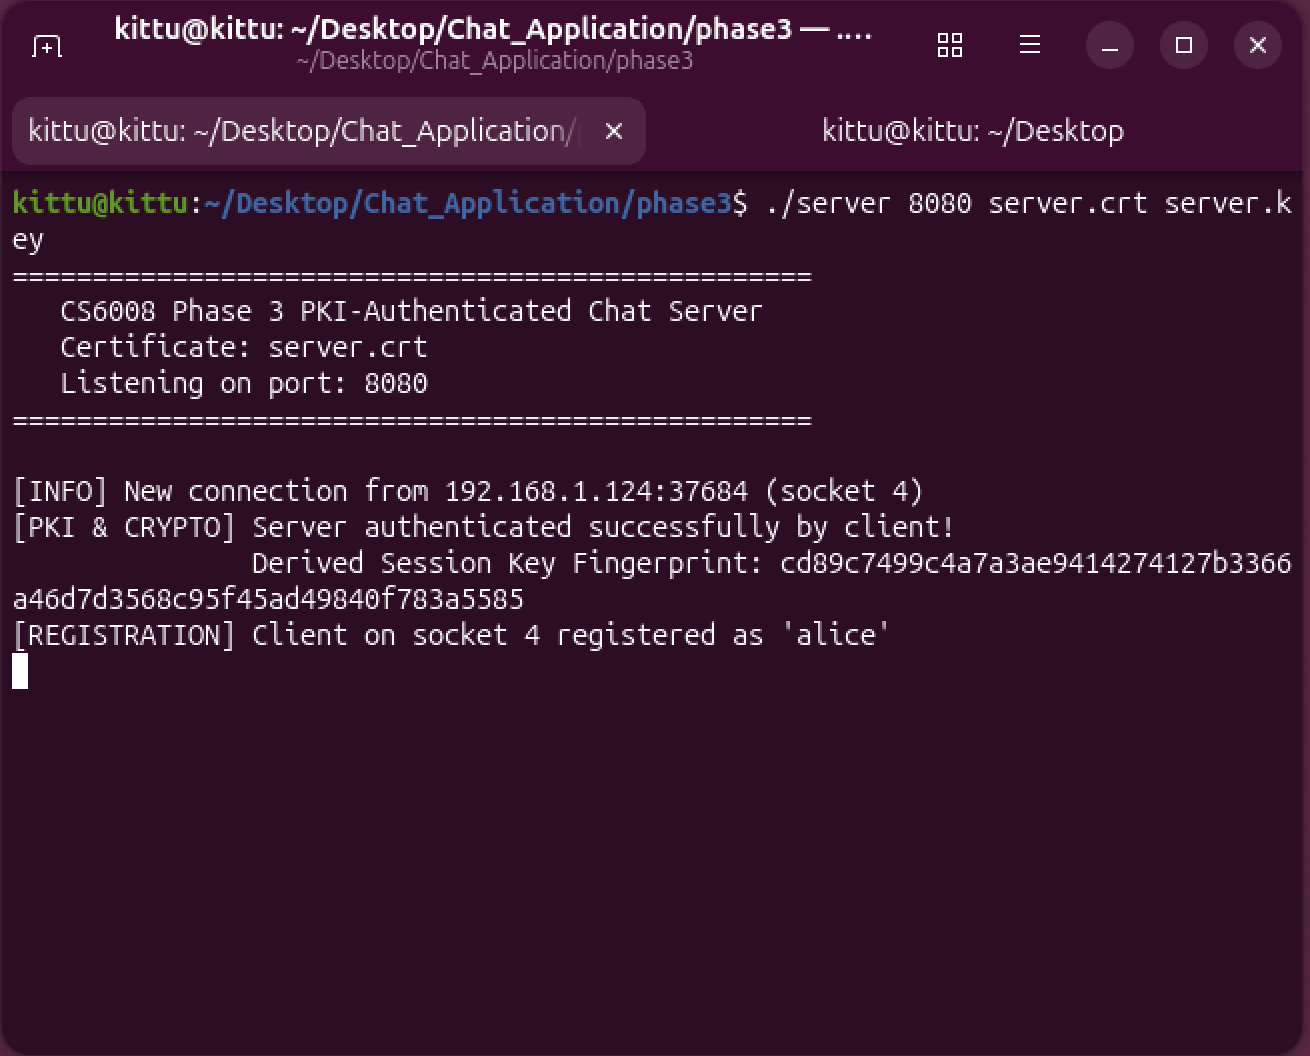
\includegraphics[width=\linewidth]{phase3_legitimate_server.png}
        \caption{Phase 3: Server confirming authentication.}
        \label{fig:phase3_legit_server}
    \end{minipage}
\end{figure}

\subsection{Defeating MITM Attacks}
We evaluated two distinct attack vectors using our updated \texttt{mallory\_proxy}:

\subsubsection{Test 1: Mallory Self-Signed Fake Certificate}
Mallory attempts to present a forged certificate signed by an untrusted CA. As shown in Figures \ref{fig:phase3_fake_client} and \ref{fig:phase3_fake_mallory}, the client detects the untrusted certificate chain, halts execution with \texttt{[PKI VALIDATION FAILED]}, and closes the socket before exposing any DH parameters.

\begin{figure}[H]
    \centering
    \begin{minipage}{0.48\textwidth}
        \centering
        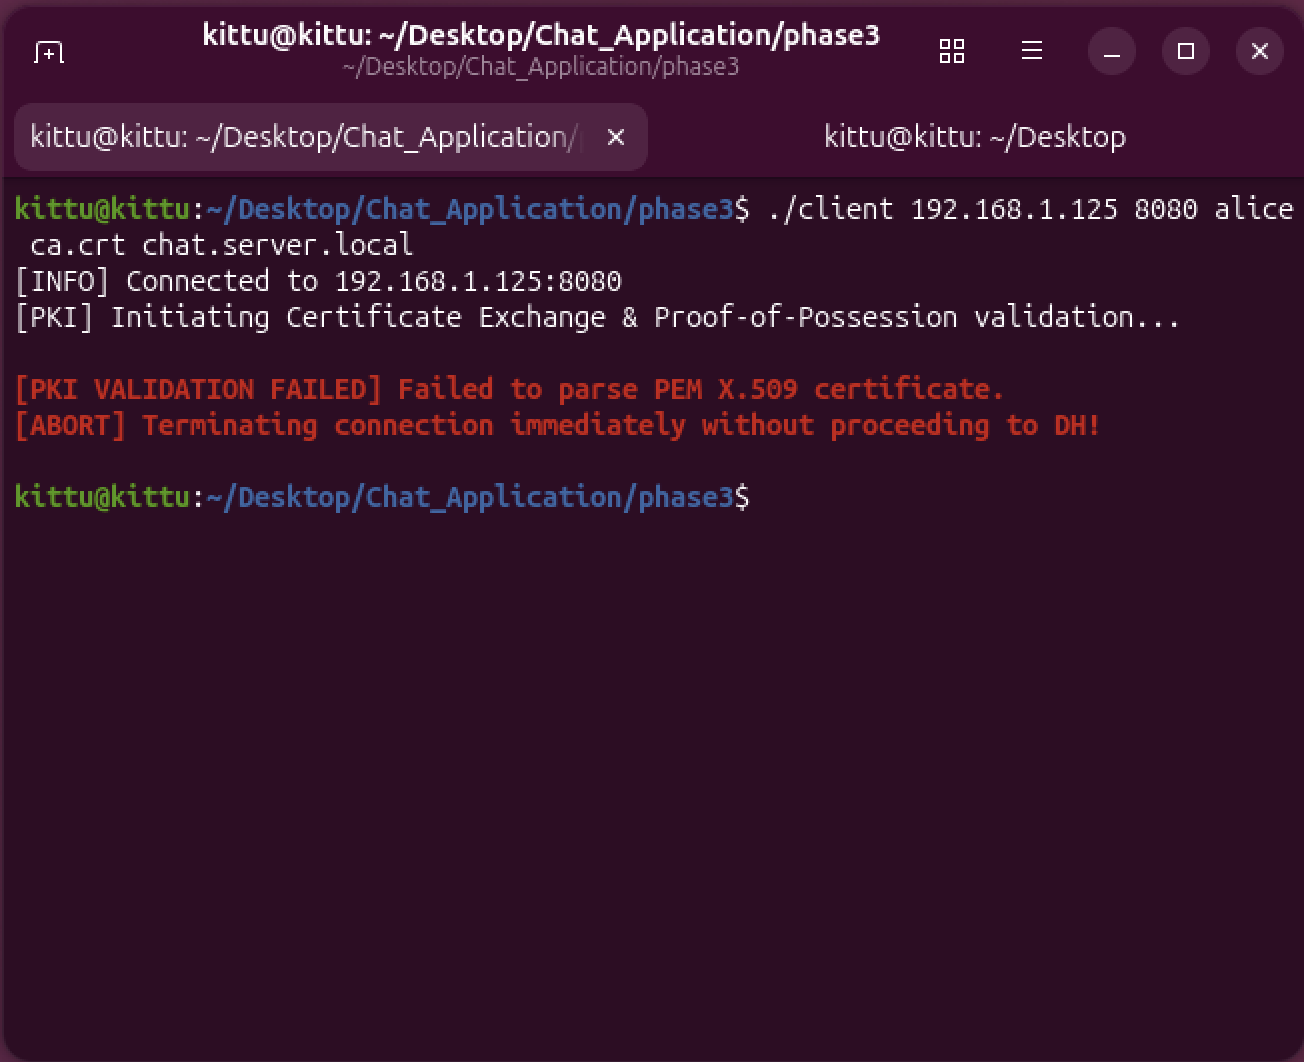
\includegraphics[width=\linewidth]{phase3_untrusted_cert_client_fail.png}
        \caption{Phase 3: Client rejecting untrusted fake cert.}
        \label{fig:phase3_fake_client}
    \end{minipage}\hfill
    \begin{minipage}{0.48\textwidth}
        \centering
        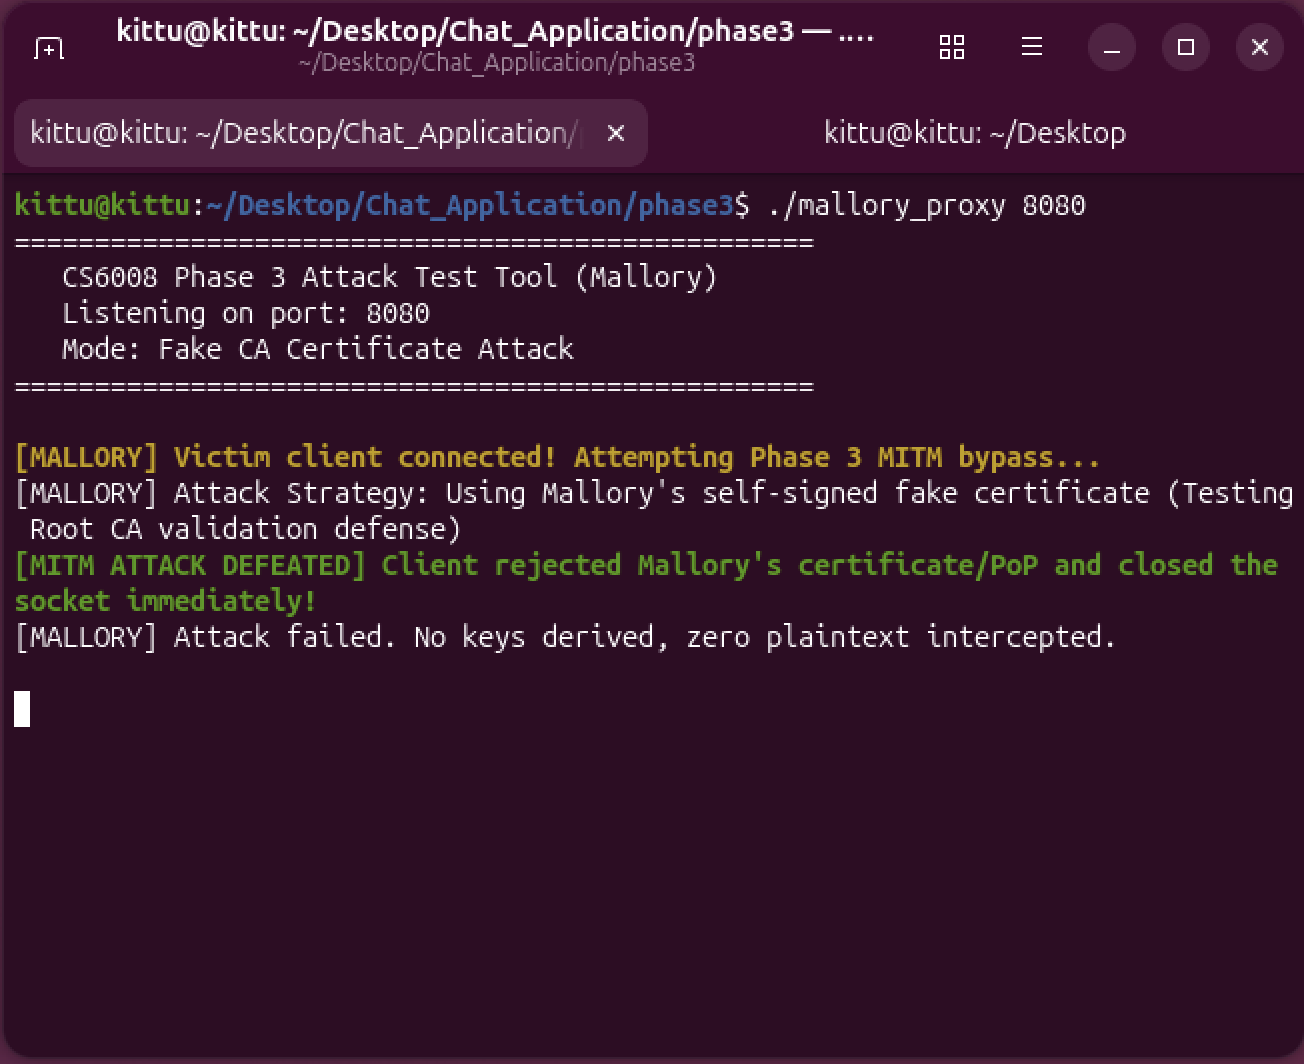
\includegraphics[width=\linewidth]{phase3_untrusted_cert_mallory_fail.png}
        \caption{Phase 3: Mallory logging fake cert defeat.}
        \label{fig:phase3_fake_mallory}
    \end{minipage}
\end{figure}

\subsubsection{Test 2: Mallory Replaying Stolen Legitimate Certificate}
Mallory presents the authentic, CA-signed \texttt{server.crt} but lacks \texttt{server.key}. When challenged to sign $(N_{\text{client}} \mathbin{\Vert} \text{DH\_Pub})$, Mallory must forge the signature using her own private key. The client extracts the authentic public key from \texttt{server.crt}, and the signature verification fails (Figures \ref{fig:phase3_pop_client} and \ref{fig:phase3_pop_mallory}).

\begin{figure}[H]
    \centering
    \begin{minipage}{0.48\textwidth}
        \centering
        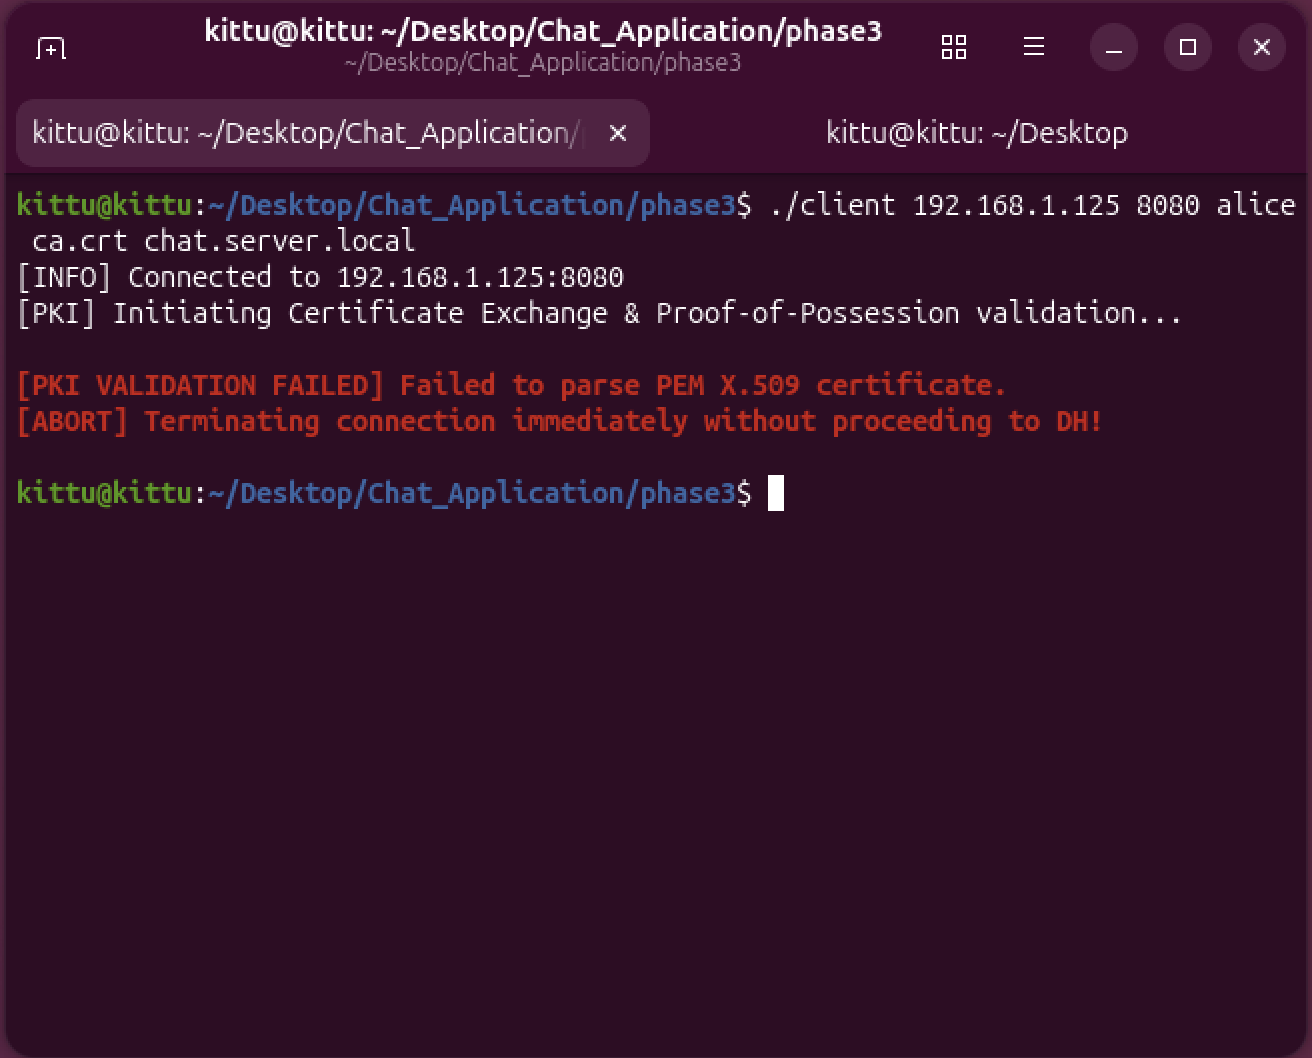
\includegraphics[width=\linewidth]{phase3_stolen_cert_pop_bypass_client_fail.png}
        \caption{Phase 3: Client rejecting invalid PoP signature.}
        \label{fig:phase3_pop_client}
    \end{minipage}\hfill
    \begin{minipage}{0.48\textwidth}
        \centering
        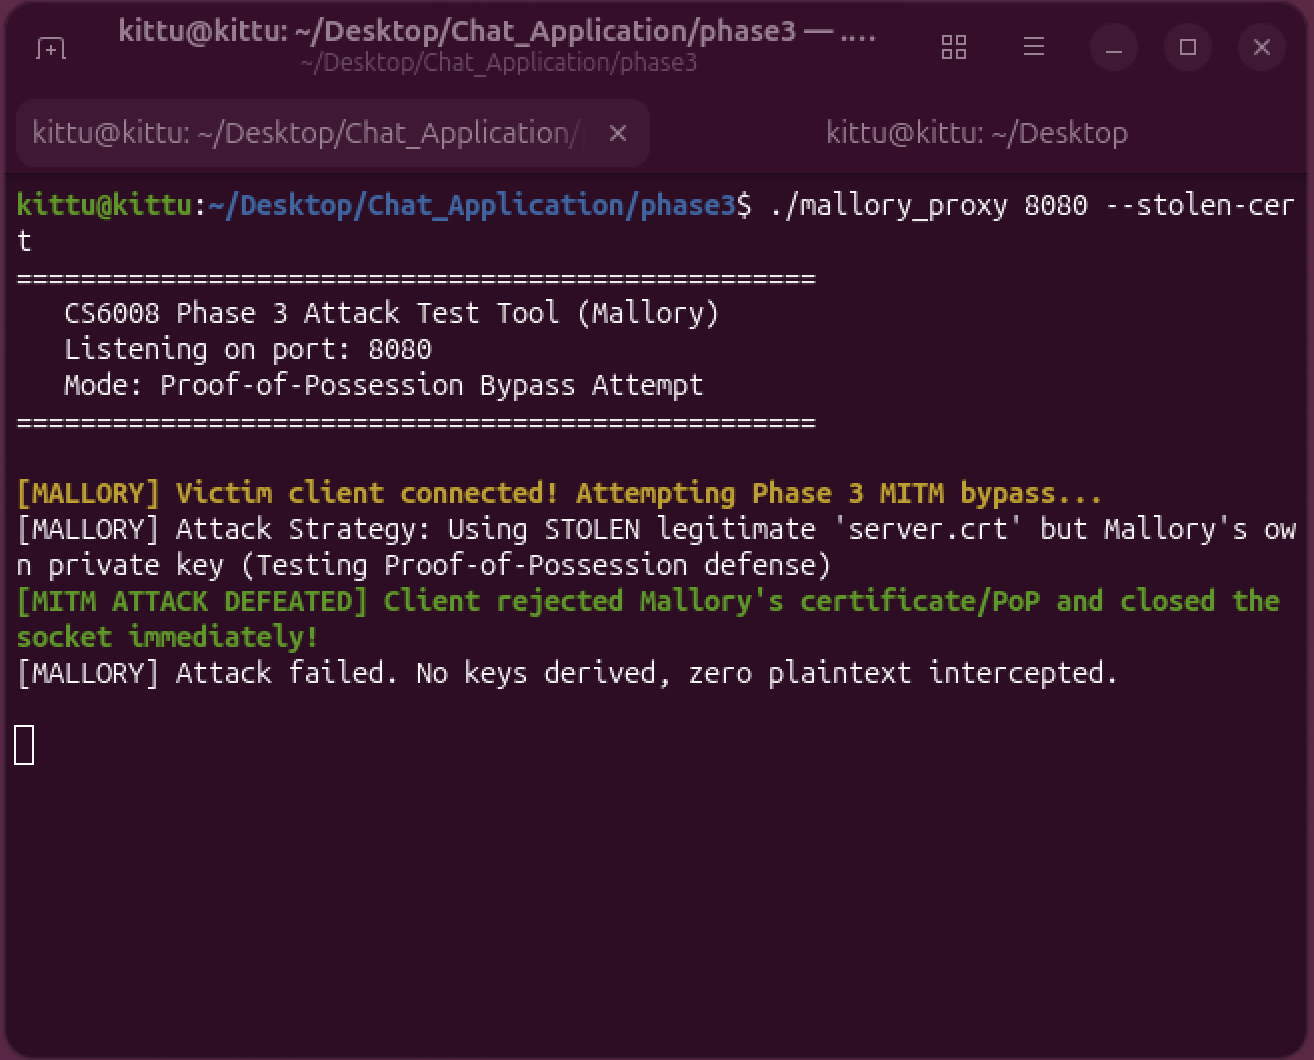
\includegraphics[width=\linewidth]{phase3_stolen_cert_pop_bypass_mallory_fail.png}
        \caption{Phase 3: Mallory logging PoP defeat.}
        \label{fig:phase3_pop_mallory}
    \end{minipage}
\end{figure}

\section{Phase 4: End-to-End Encryption (E2E)}

\subsection{Limitations of Link-Level Security}
In Phases 2 and 3, encryption terminated at the server. While protected against external eavesdroppers, the central server had full access to plaintext, representing a single point of compromise and insider threat.

\subsection{E2E Handshake \& Wire-Level Tagging}
Phase 4 implements direct client-to-client Diffie--Hellman key agreement multiplexed across the chat server using standardized wire tags:
\begin{itemize}
    \item \texttt{\_\_E2E\_INIT\_\_<Alice\_DH\_Pub>}
    \item \texttt{\_\_E2E\_ACK\_\_<Bob\_DH\_Pub>}
    \item \texttt{\_\_E2E\_MSG\_\_<Encrypted\_Payload\_Hex>}
\end{itemize}

\subsection{Double-Layered Encryption}
Messages transmitted between peers undergo two nested layers of AES-256-GCM authenticated encryption:
\begin{enumerate}
    \item \textbf{Inner Layer (E2E):} Plaintext is encrypted with the direct peer key $K_{\text{E2E}}$ and wrapped in \texttt{\_\_E2E\_MSG\_\_}.
    \item \textbf{Outer Layer (Transport):} The tagged message is encrypted under the hop-by-hop link key $K_{\text{Link}}$ established with the server.
\end{enumerate}

\begin{figure}[H]
    \centering
    \begin{minipage}{0.48\textwidth}
        \centering
        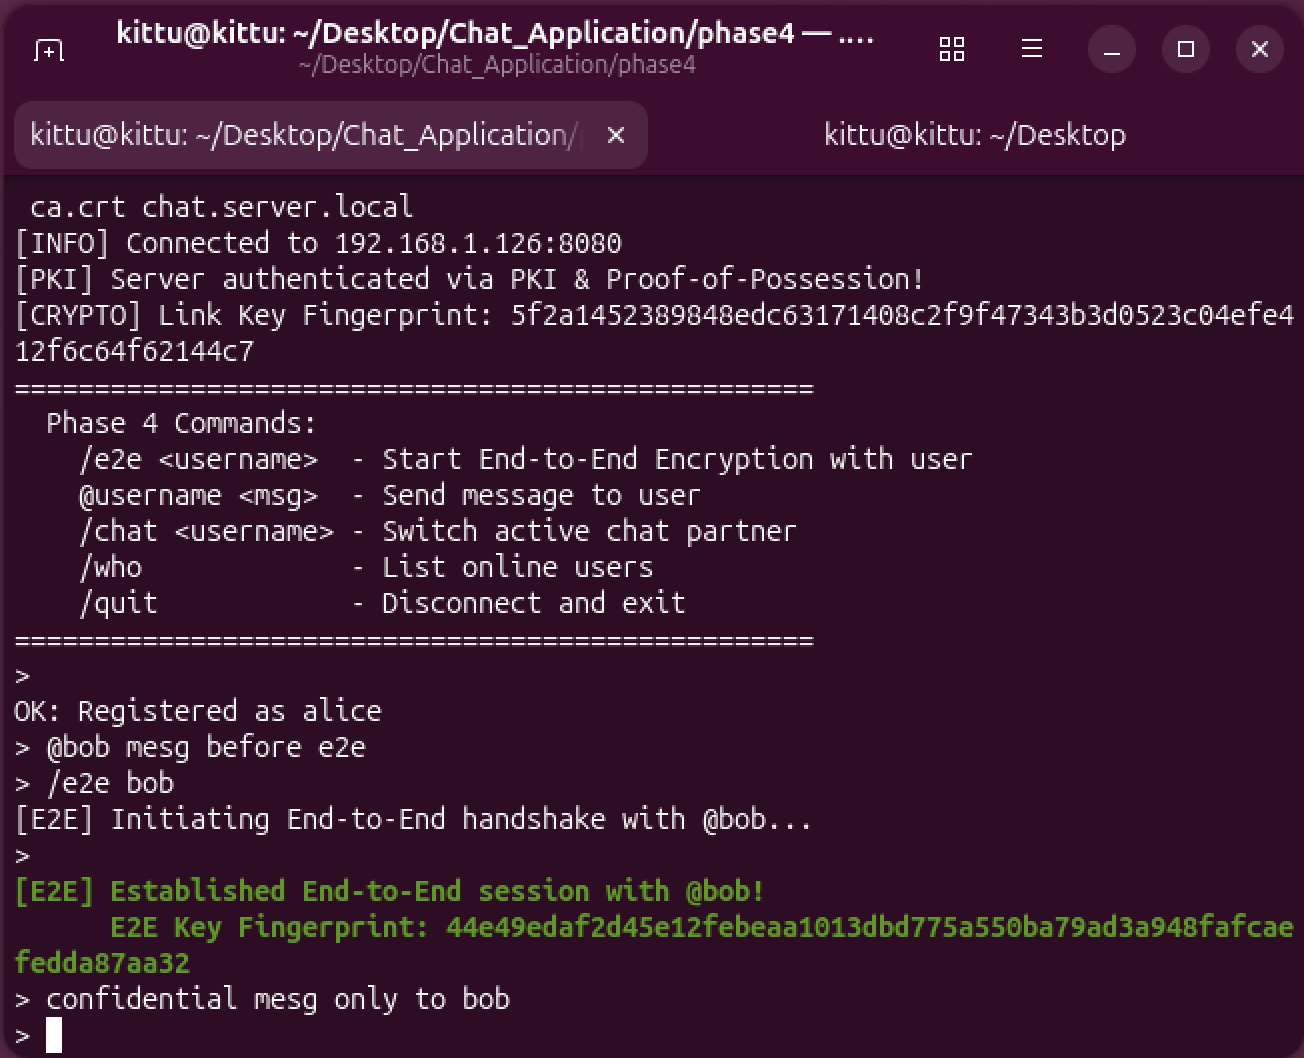
\includegraphics[width=\linewidth]{phase4_alice_e2e_init.png}
        \caption{Phase 4: Alice establishing E2E key session.}
        \label{fig:phase4_alice}
    \end{minipage}\hfill
    \begin{minipage}{0.48\textwidth}
        \centering
        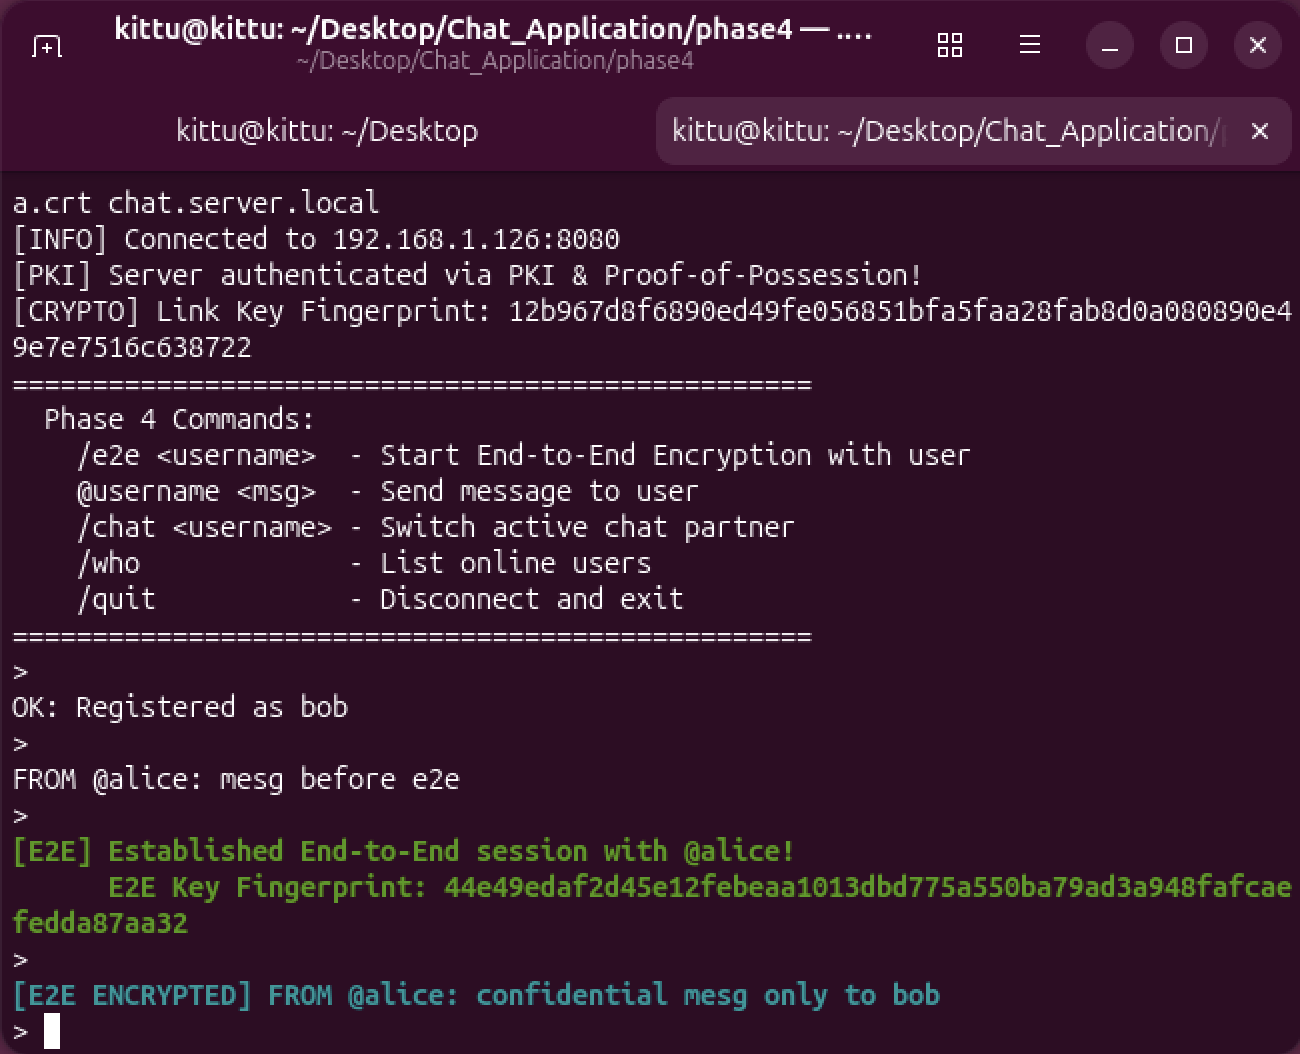
\includegraphics[width=\linewidth]{phase4_bob_e2e_receive.png}
        \caption{Phase 4: Bob matching E2E key \& decrypting.}
        \label{fig:phase4_bob}
    \end{minipage}
\end{figure}

\subsection{Verification of Server Blindness}
To prove zero-knowledge server blindness, we compared server relay logs before and after triggering \texttt{/e2e bob}.

\begin{figure}[H]
    \centering
    \begin{minipage}{0.48\textwidth}
        \centering
        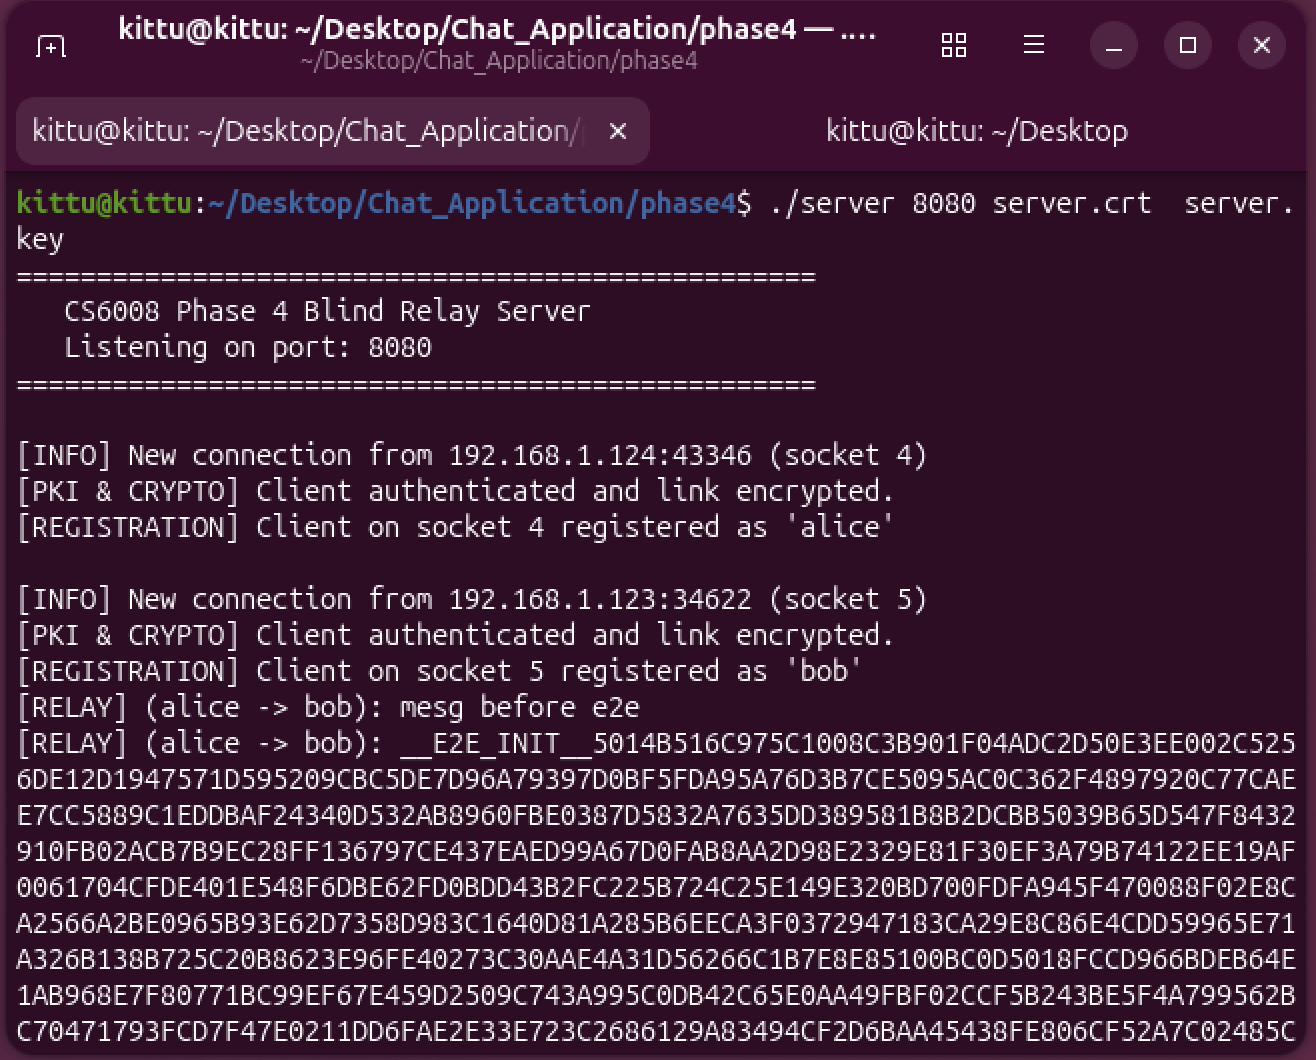
\includegraphics[width=\linewidth]{phase4_server_blind_relay_1.png}
        \caption{Phase 4: Server relay (Pre-E2E vs \texttt{\_\_E2E\_INIT\_\_}).}
        \label{fig:phase4_server1}
    \end{minipage}\hfill
    \begin{minipage}{0.48\textwidth}
        \centering
        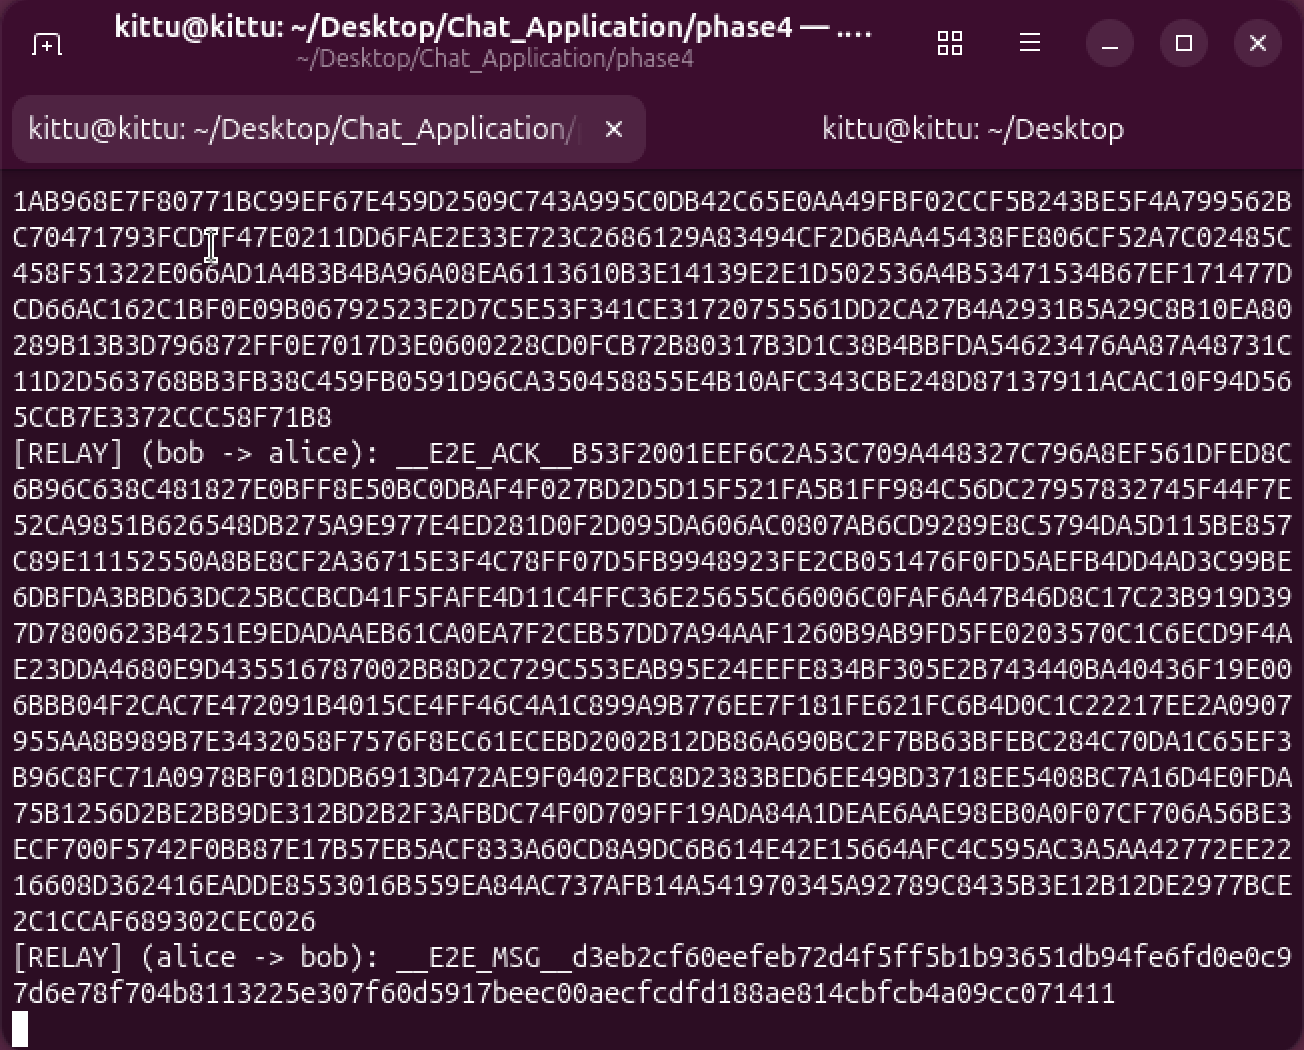
\includegraphics[width=\linewidth]{phase4_server_blind_relay_2.png}
        \caption{Phase 4: Server relay (\texttt{\_\_E2E\_ACK\_\_} \& \texttt{\_\_E2E\_MSG\_\_}).}
        \label{fig:phase4_server2}
    \end{minipage}
\end{figure}

As shown in Figures \ref{fig:phase4_server1} and \ref{fig:phase4_server2}, before E2E initiation the server logged readable chat text (\texttt{"mesg before e2e"}). After \texttt{/e2e bob}, the server logs exclusively opaque, uncrackable ciphertext (\texttt{\_\_E2E\_MSG\_\_3deb2cf60e...}), proving complete server blindness.

\section{Phase 5: Forward Secrecy via Key Rotation}

\subsection{Threat Model \& Value of Forward Secrecy}
\textbf{Theoretical Rationale:} In Phase 4, a single static symmetric key $K_{\text{E2E}}$ protects the entire duration of an E2E session. If an adversary passively records encrypted network traffic for days or months and later compromises the client host (recovering $K_{\text{E2E}}$ from disk or memory), the adversary can retroactively decrypt the entire recorded session history.

Forward Secrecy ensures that compromise of a current long-term or session key does \textbf{not} compromise past session keys. Each conversation epoch is encrypted under an independent, short-lived ephemeral key that is permanently destroyed upon rotation.

\subsection{Ratchet Mechanism \& Memory Zeroization}
Phase 5 introduces automated, periodic key rotation:
\begin{enumerate}
    \item \textbf{Periodic Timer:} A background thread executes an ephemeral Diffie--Hellman re-exchange every 60 seconds (or immediately via \texttt{/rekey}).
    \item \textbf{Memory Cleansing:} Once a new session key is derived, the previous key material and DH private exponents are immediately overwritten in RAM using \texttt{OPENSSL\_cleanse()} to prevent extraction via memory dumps or cold-boot attacks.
\end{enumerate}

\subsection{Simultaneous Rekey Collision Avoidance}
\textbf{Design Justification:} If Alice and Bob trigger key rotation at the exact same instant, both will transmit \texttt{\_\_E2E\_INIT\_\_} simultaneously, risking race conditions and key desynchronization.

We resolve this through a deterministic \textbf{lexicographical tie-breaker}:
\begin{itemize}
    \item When receiving an \texttt{\_\_E2E\_INIT\_\_} while in the \texttt{AWAITING\_ACK} state, clients compare usernames (\texttt{username\_self < username\_peer}).
    \item The client with the lexicographically higher username proceeds as the initiator; the lower-ranked client drops its pending init and yields, immediately replying with \texttt{\_\_E2E\_ACK\_\_}.
\end{itemize}

\subsection{Empirical Rotation Verification}
We verified three consecutive key rotations over live sessions.

\begin{figure}[H]
    \centering
    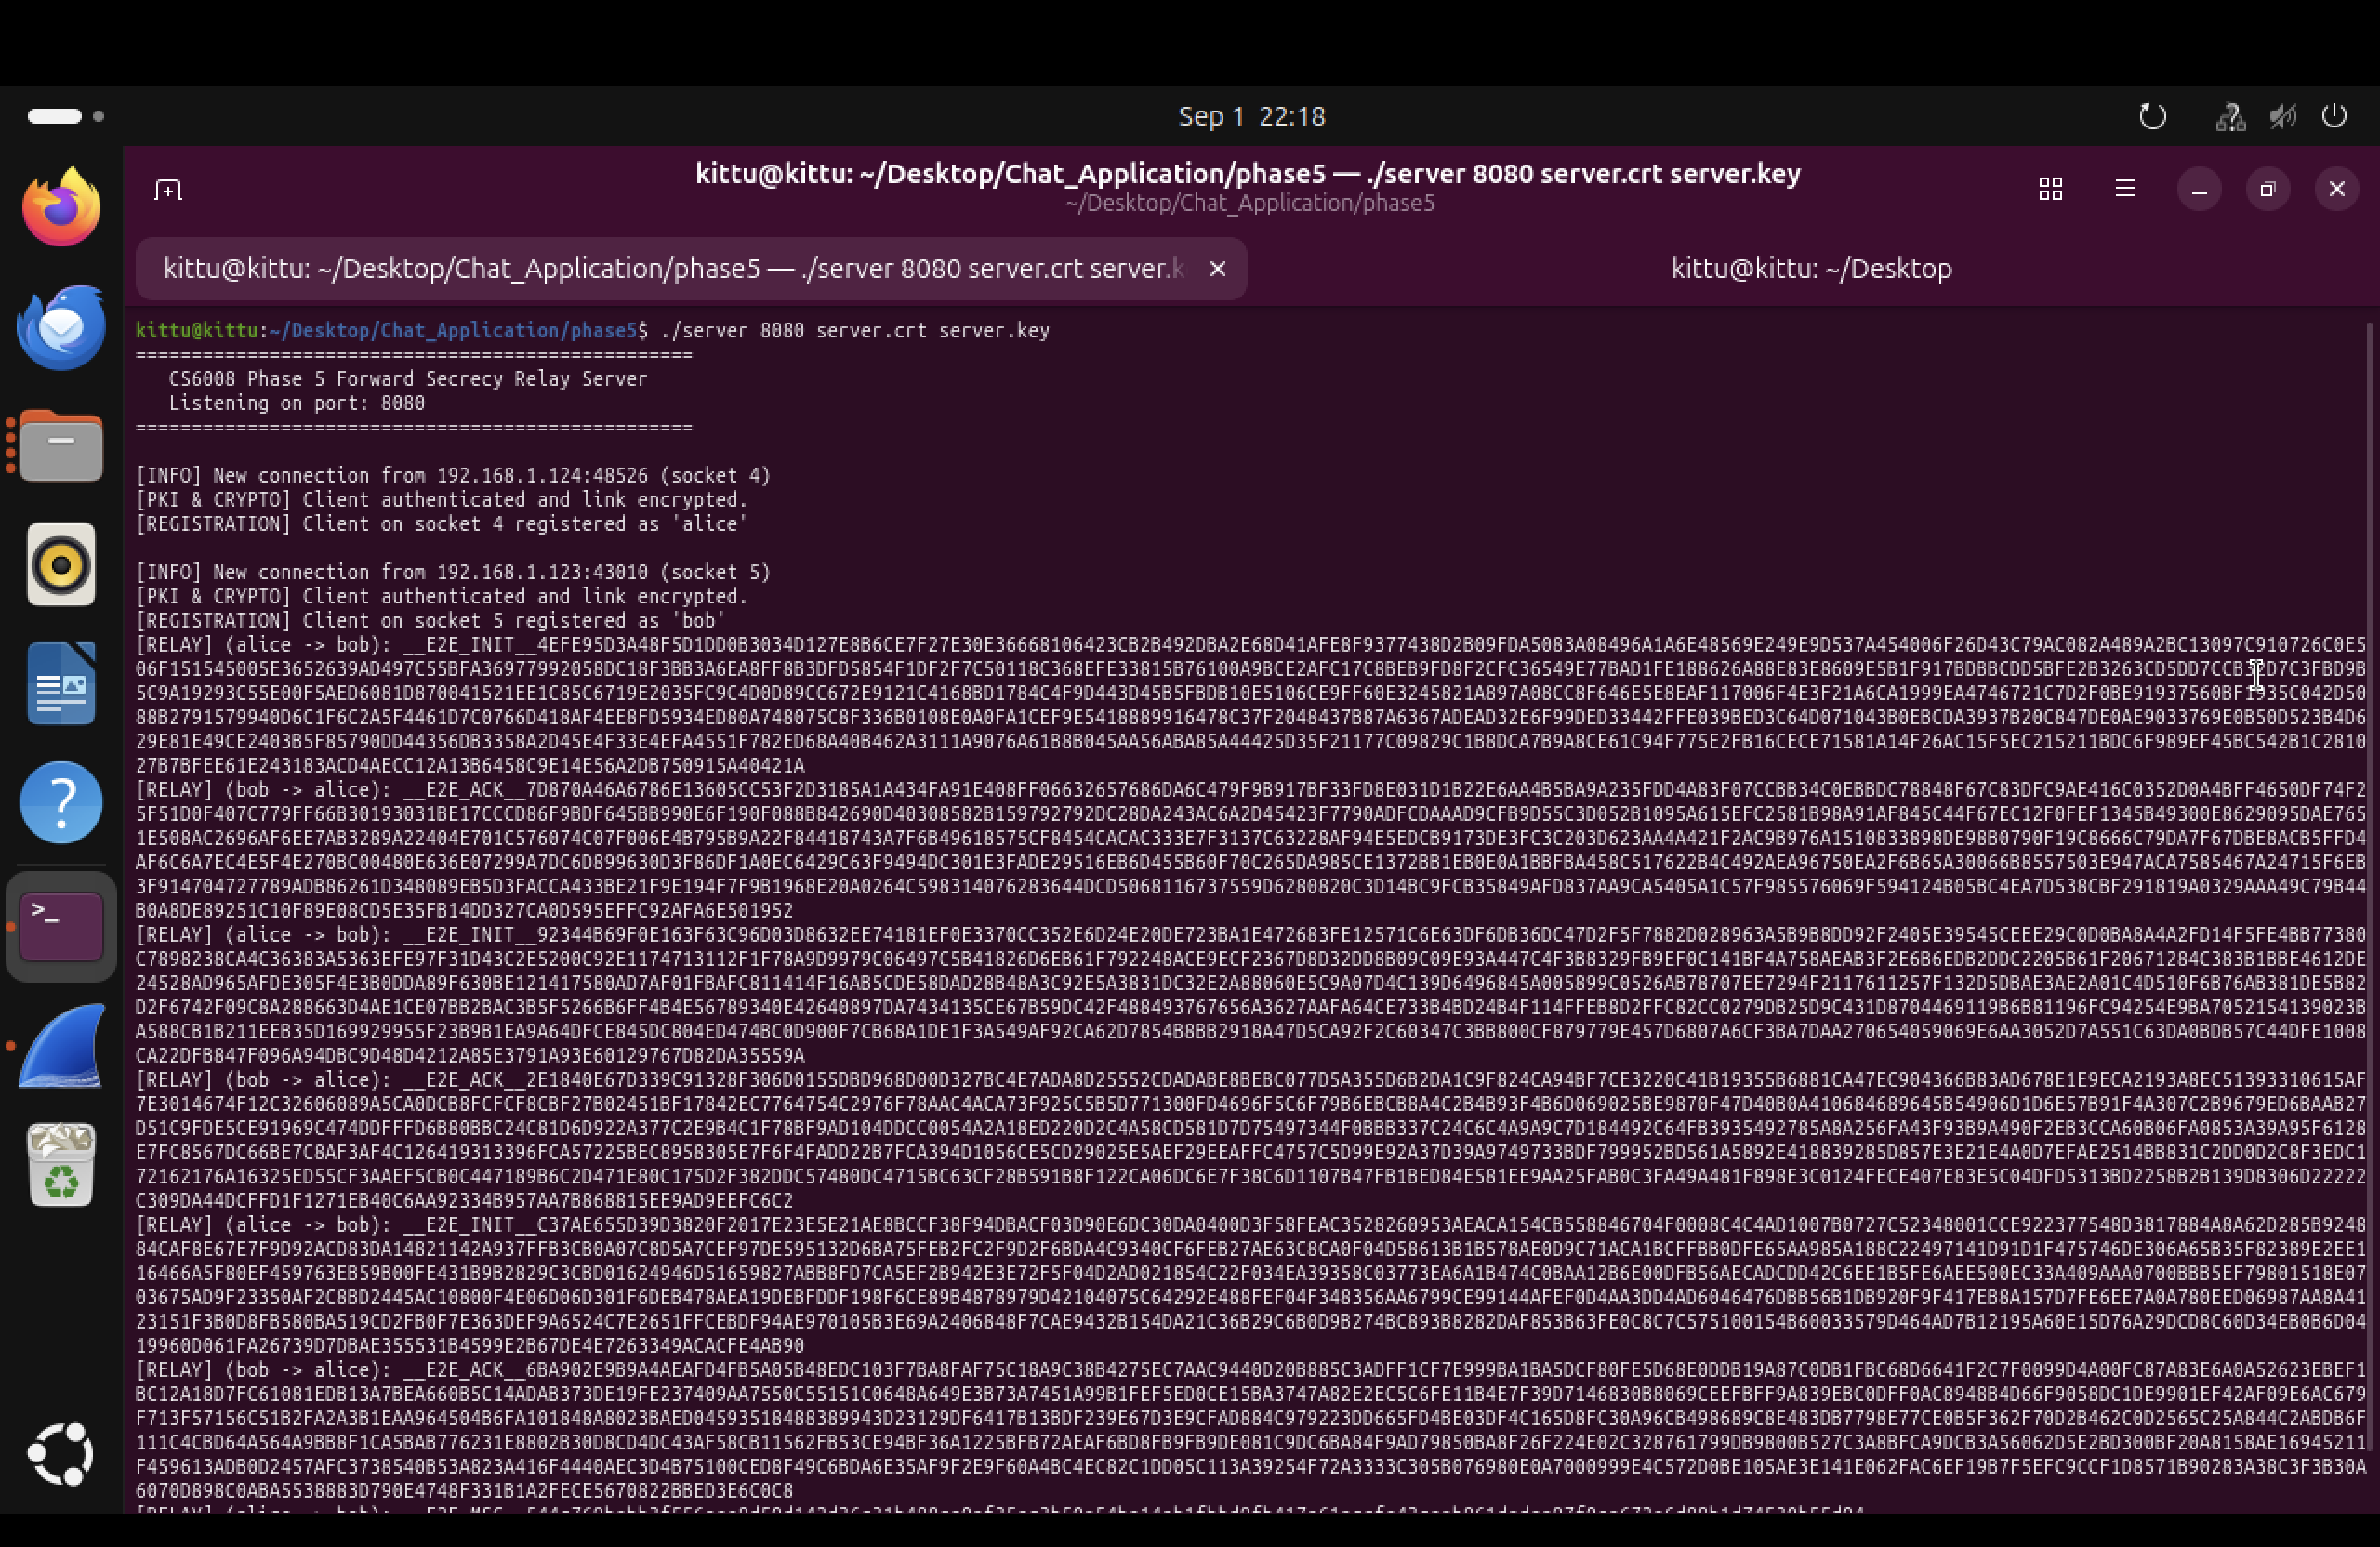
\includegraphics[width=0.75\linewidth]{phase5_server_rotations.png}
    \caption{Phase 5: Server relaying multiple periodic E2E rekey handshakes.}
    \label{fig:phase5_server}
\end{figure}

\begin{figure}[H]
    \centering
    \begin{minipage}{0.48\textwidth}
        \centering
        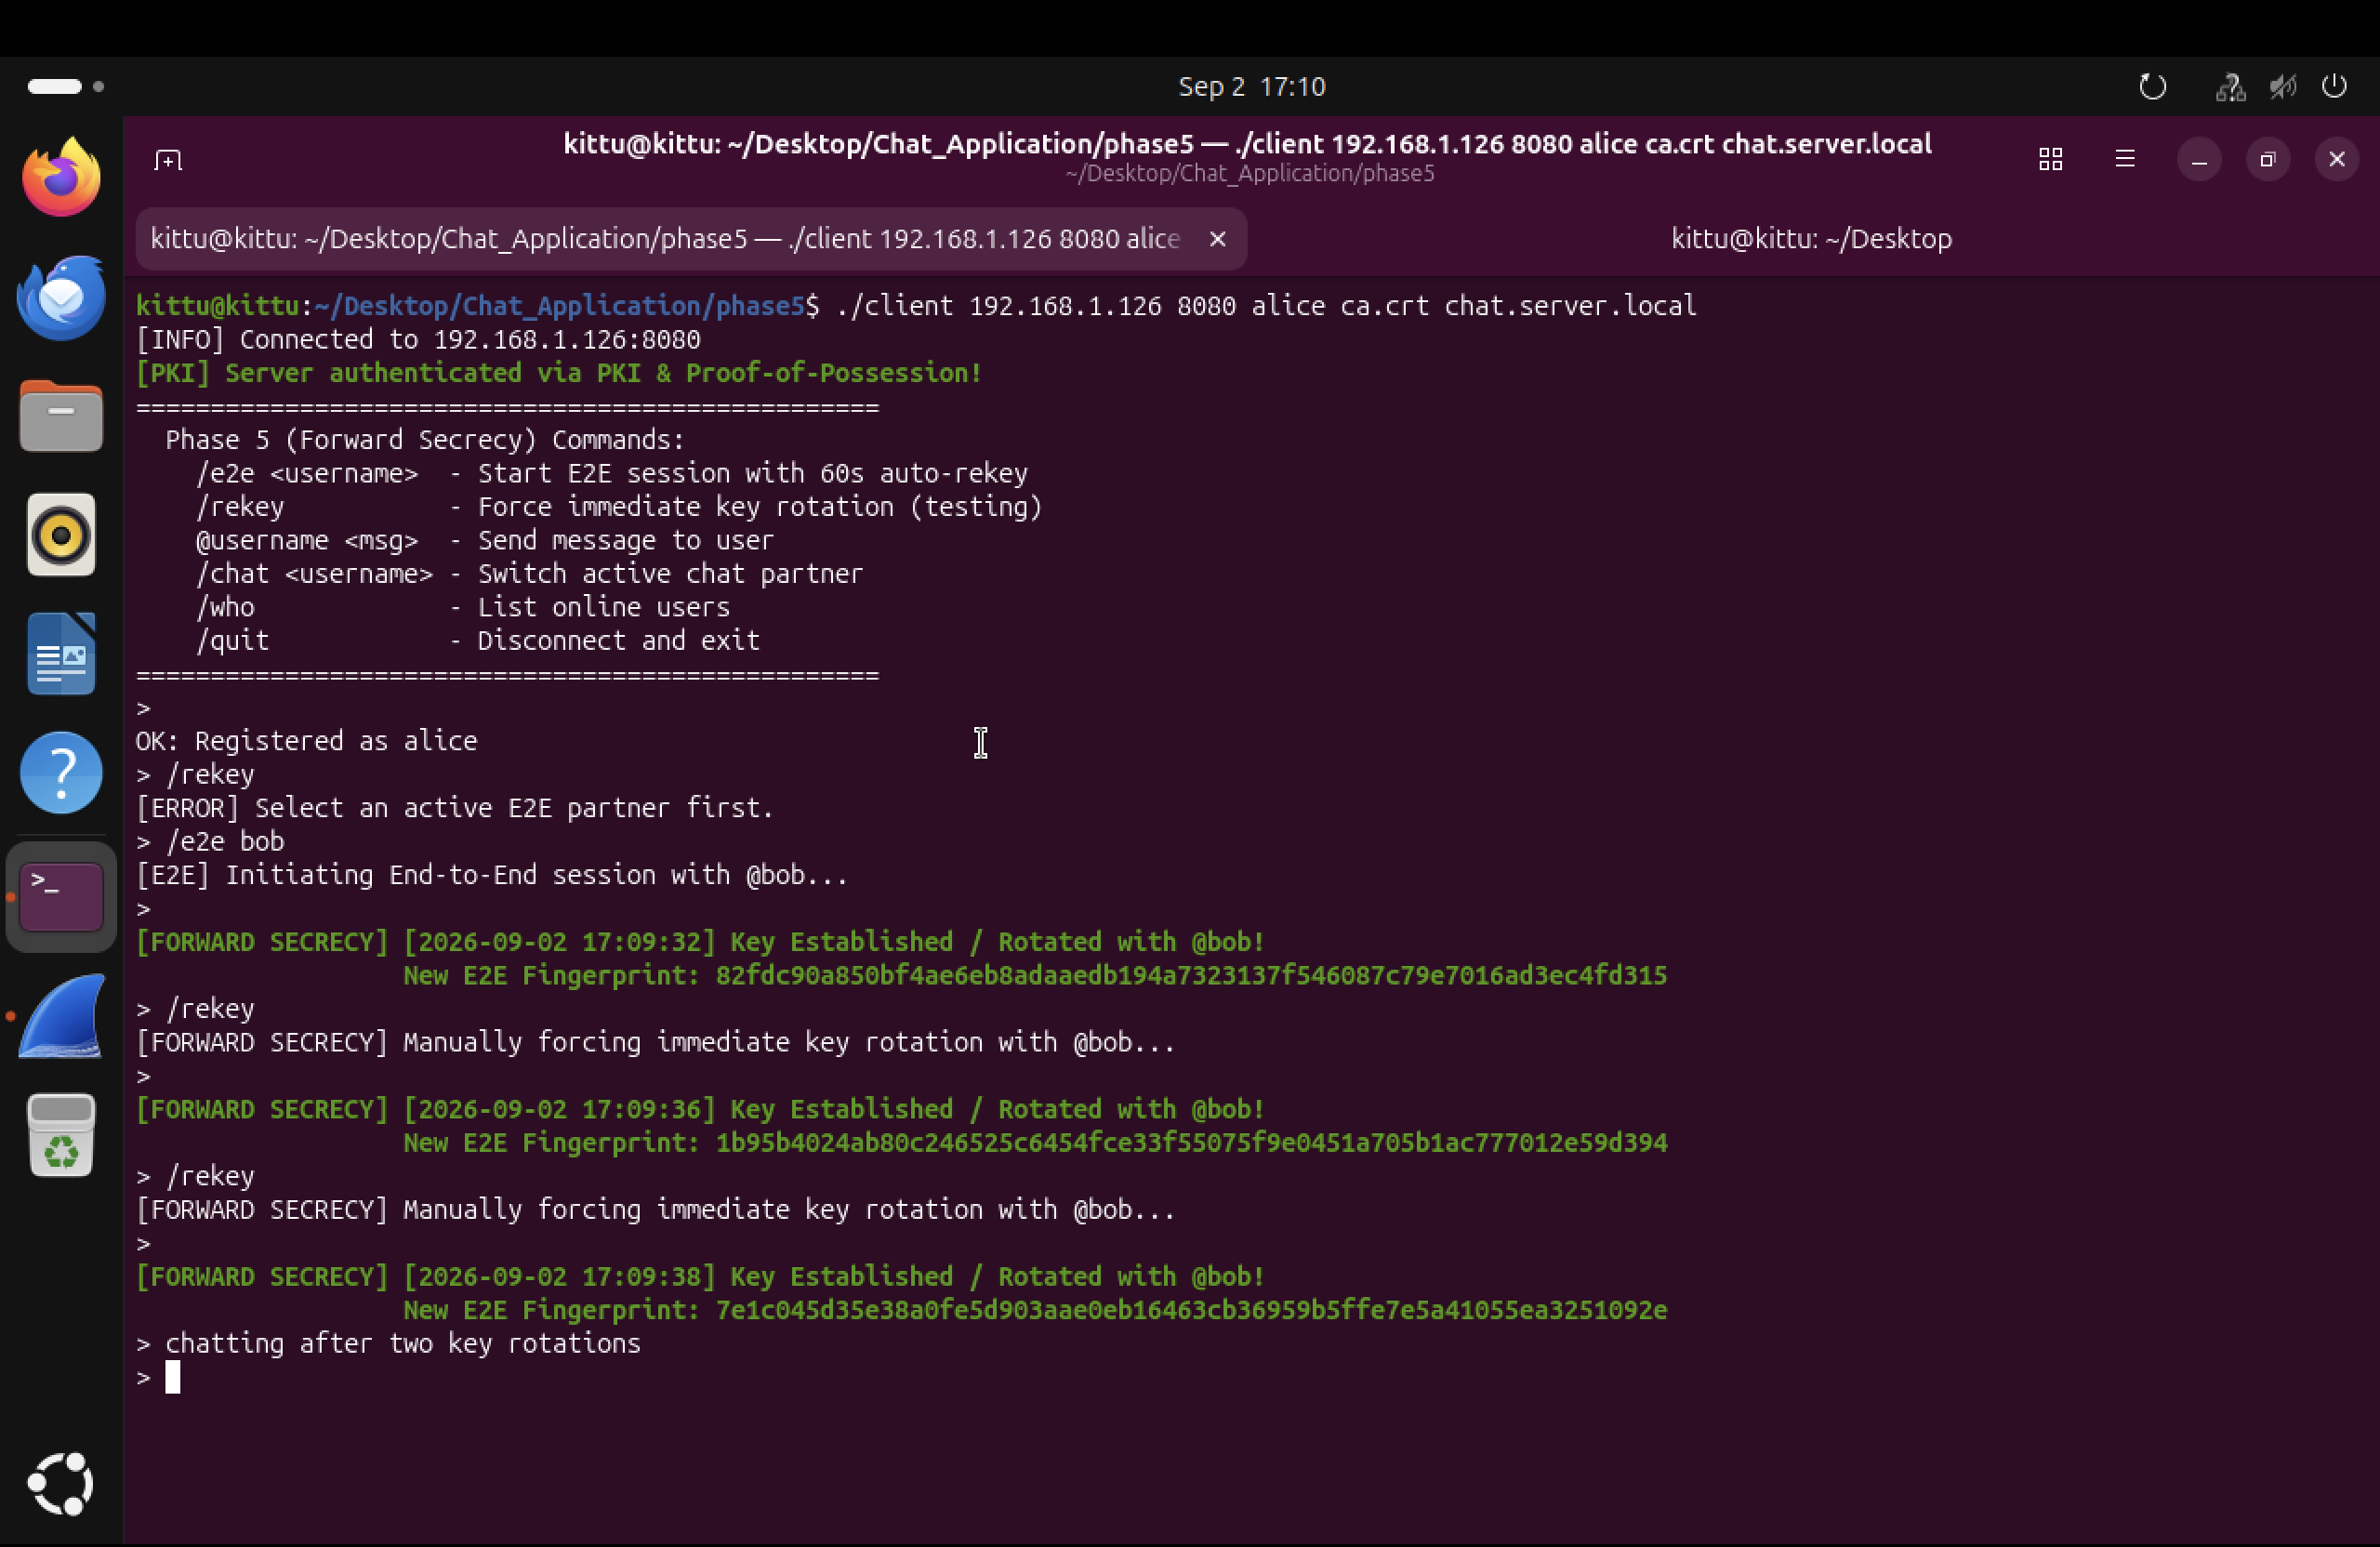
\includegraphics[width=\linewidth]{phase5_alice_rotations.png}
        \caption{Phase 5: Alice log showing 2 rotations.}
        \label{fig:phase5_alice}
    \end{minipage}\hfill
    \begin{minipage}{0.48\textwidth}
        \centering
        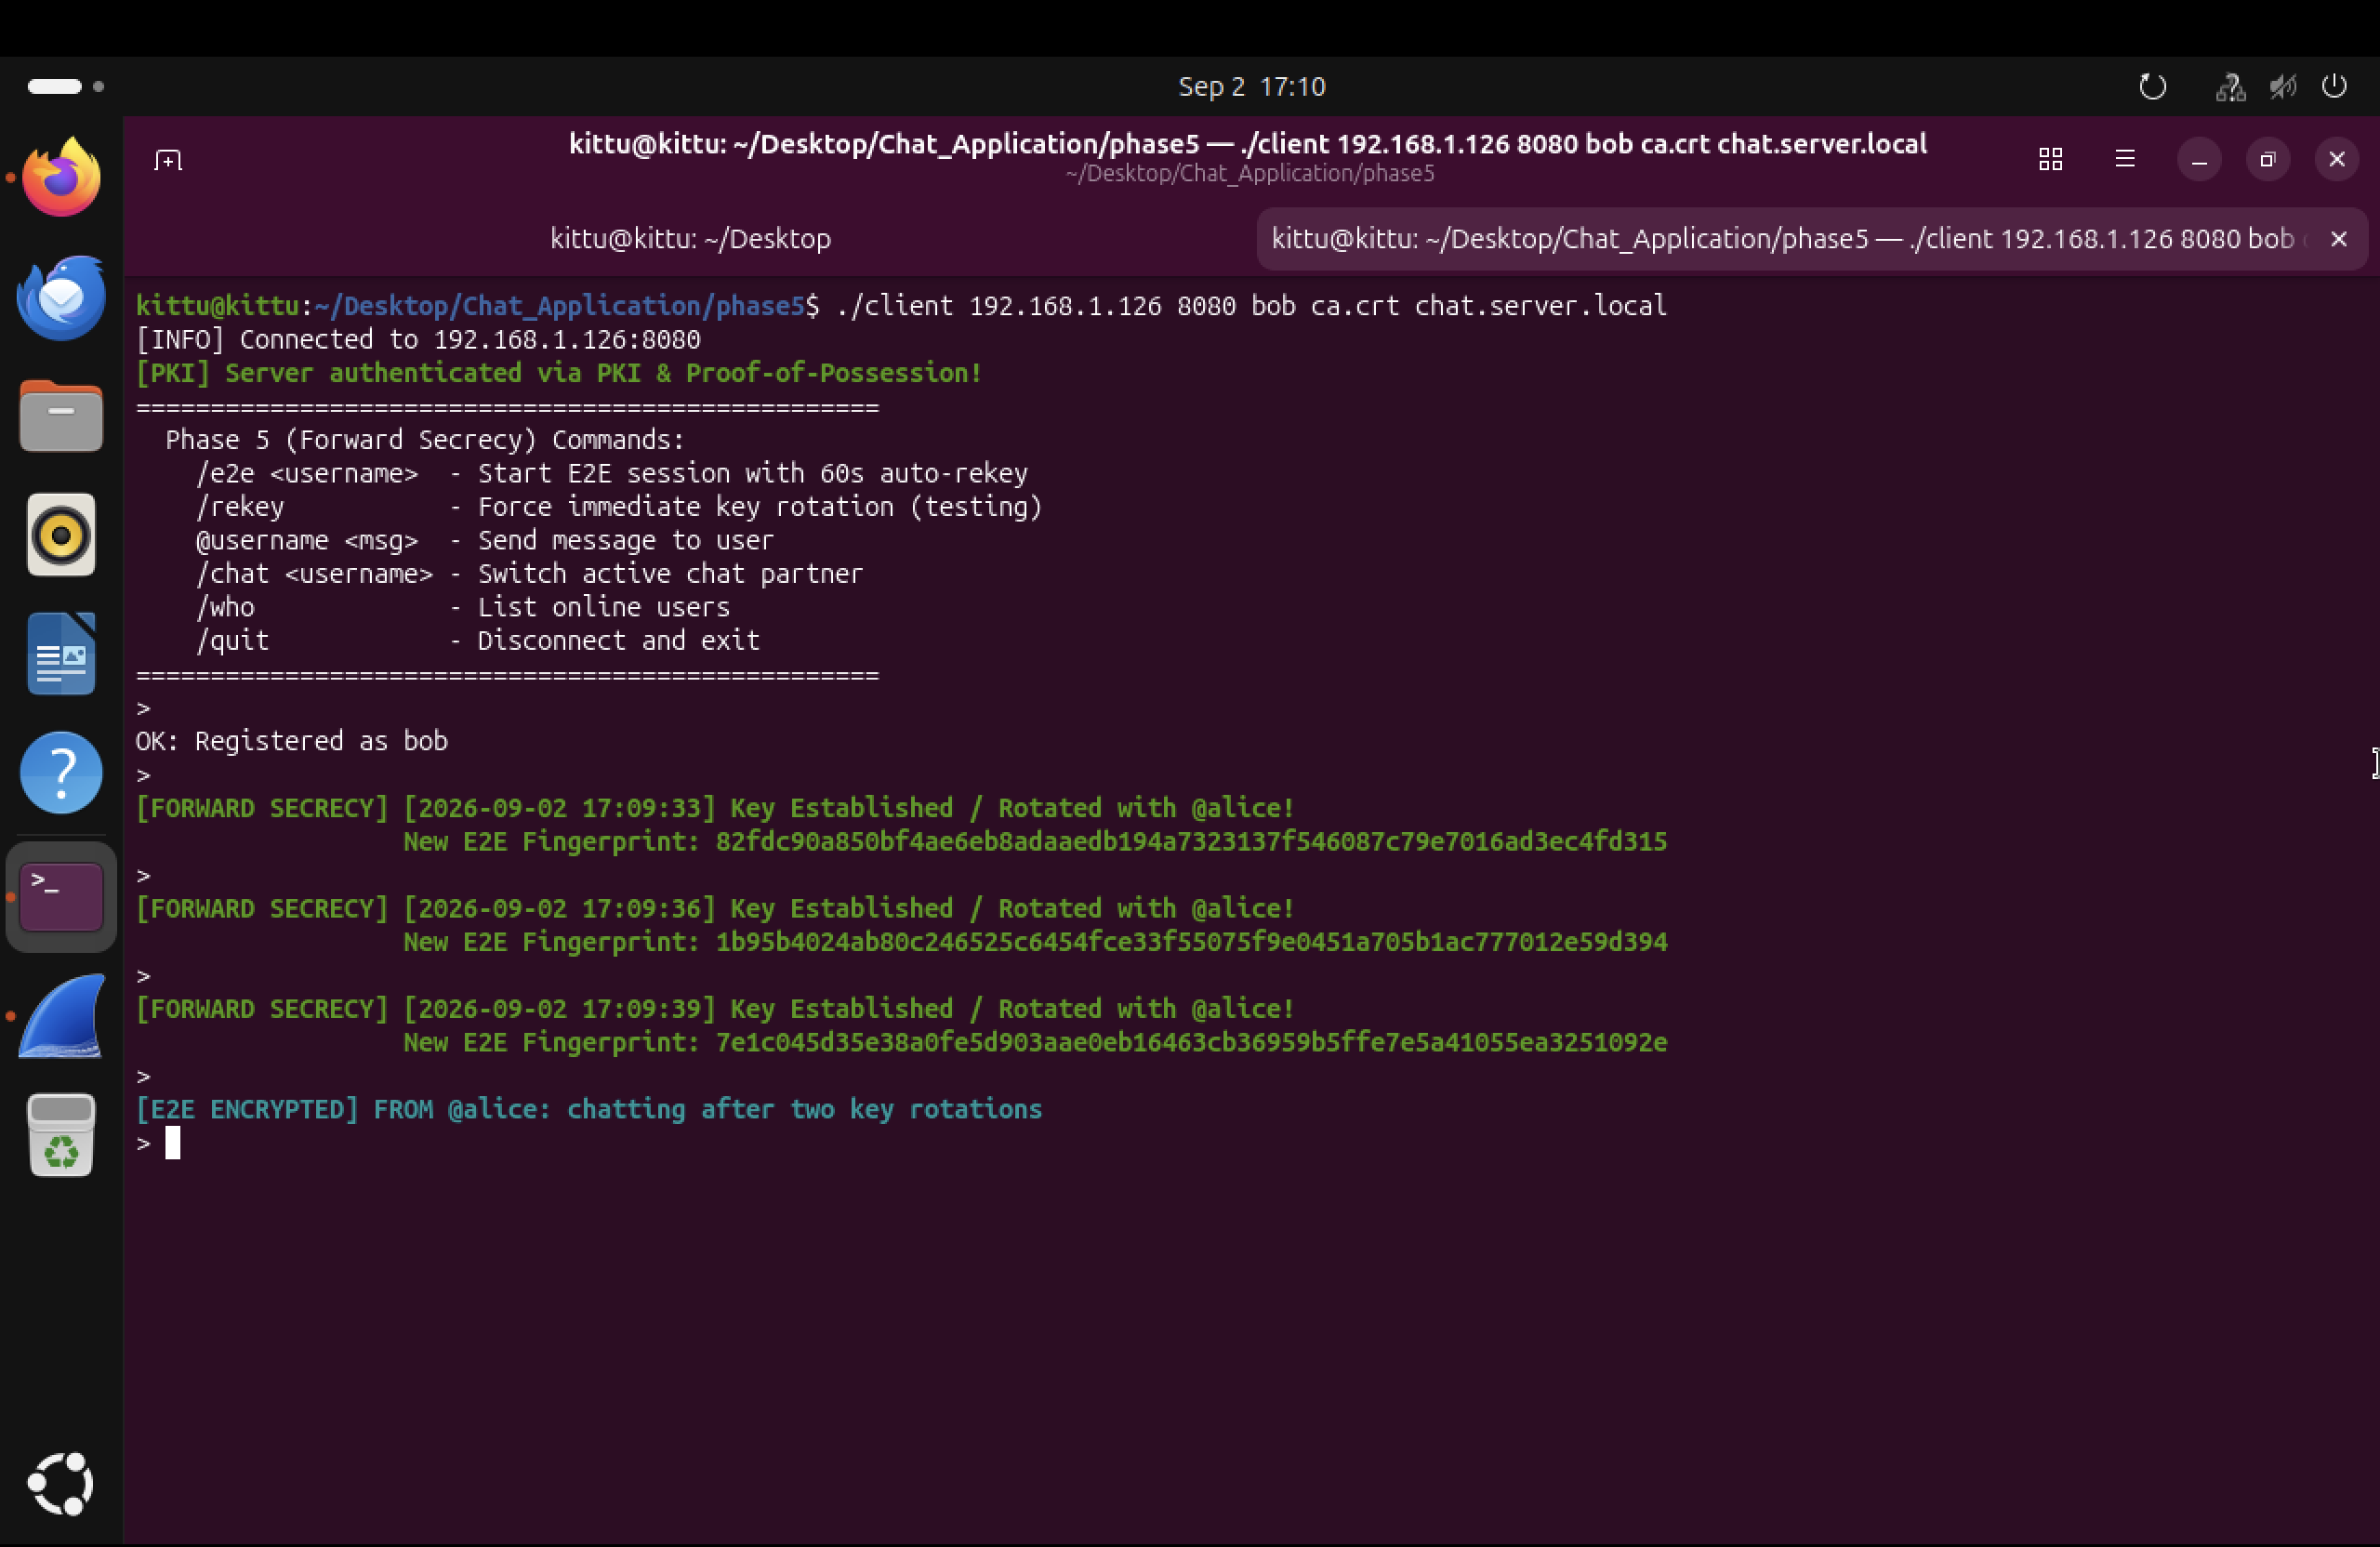
\includegraphics[width=\linewidth]{phase5_bob_rotations_and_chat.png}
        \caption{Phase 5: Bob log showing matching keys.}
        \label{fig:phase5_bob}
    \end{minipage}
\end{figure}

As evidenced in Figures \ref{fig:phase5_server}, \ref{fig:phase5_alice}, and \ref{fig:phase5_bob}, both clients agree on the updated fingerprint after each rotation (\texttt{82fdc9...} $\rightarrow$ \texttt{1b95b4...} $\rightarrow$ \texttt{7e1c04...}), and messages sent after multiple rotations decrypt flawlessly.

\section{Conclusion}
Through the iterative development of Phases 1 to 5, we have systematically engineered a robust, modern cryptographic communication system. Starting from a vulnerable plaintext baseline, we incorporated mathematical key exchange, authenticated symmetric encryption, rigorous PKI validation, zero-knowledge blind relaying, and ratcheted forward secrecy, validating each security guarantee through empirical network captures and adversarial testing.

\appendix
\section{Generative AI Usage \& Prompt Log}
In accordance with assignment policy, LLM assistance was utilized for boilerplate generation and conceptual planning. The detailed prompt sequence is documented below:
\begin{enumerate}
    \item \textit{"How should I plan the structure of the code files so that as I finish the phases one-by-one while maintaining the modularity of the code files."}
    \item \textit{"Provide the OpenSSL EVP code snippet for AES-256-GCM encryption with 12-byte IV and 16-byte authentication tag retrieval."}
    \item \textit{"How to perform X.509 certificate verification against a Root CA store in C++ using OpenSSL low-level functions without using SSL\_CTX?"}
    \item \textit{"Create readme.md files for each phase's folder explaining the respective folder code structure and the basic commands used for getting results."}
    \item \textit{"Using the Screenshots uploaded, create a template for a latex file for the report."}
\end{enumerate}

\end{document}
